% Complete manuscript assembled by scripts/assemble_manuscript.py.
% Editable sources: manuscript_template.tex, sections/, and tables/.
\documentclass[preprint,12pt,a4paper]{elsarticle}
\usepackage[T1]{fontenc}
\usepackage[margin=25mm]{geometry}
\usepackage{amsmath,amssymb,booktabs,graphicx,array,microtype}
\usepackage[section]{placeins}
\usepackage{xurl}
\usepackage[hidelinks]{hyperref}
\setlength{\emergencystretch}{3em}
\setcounter{topnumber}{3}
\setcounter{totalnumber}{5}
\renewcommand{\topfraction}{0.95}
\renewcommand{\textfraction}{0.05}
\journal{Energy and AI}
% Working draft: do not imply that a submission has already occurred.
\makeatletter
\let\ps@pprintTitle\ps@plain
\makeatother
\begin{document}
\begin{frontmatter}
\title{FedGrid-RL: Attack Resilience and Honest Update Rejection in Federated Household Battery Control}
\author{Author names and affiliations to be confirmed}
\begin{abstract}

% BEGIN SOURCE: sections/abstract.tex
Federated reinforcement learning enables household batteries to share control knowledge while retaining local operating records, but compromised participants can corrupt the shared policy. We evaluate FedGrid, an aggregation method that combines solar-capacity grouping, robust within-group filtering, norm clipping and reference-based weighting. The testbed couples residual Soft Actor-Critic (SAC) controllers with export enforcement and unbalanced power-flow simulation for 36 households. Six poisoning attacks are evaluated using Ausgrid profiles, with additional retraining and transfer experiments using the Australian Capital Territory (ACT) NextGen data. Across five Ausgrid seeds, the final configuration, which filters before clipping and increases the clipping bound, lowers observed mean annual Normalized-attack damage from \$88 to \$11 per household relative to the original configuration. The paired change is $-\$76.8\pm\$67.5$ under a descriptive 95\% Student-$t$ interval; the exact two-sided signed-rank test gives $p=0.0625$ before adjustment. Reward poisoning remains a weakness, with approximately \$112 mean annual damage in ACT retraining. In the clean FedAvg comparison, solar curtailment is approximately 69\% lower than under the self-consumption rule, whereas bill savings are modest. An analysis of aggregation coefficients shows that filter admission does not guarantee positive weight, qualifying the interpretation of low recorded rejection. Cross-partition ACT imputation and post-hoc configuration selection further limit the evidence. The results support attack-specific evaluation that distinguishes economic damage, filter admission and effective contribution.

% END SOURCE: sections/abstract.tex

\end{abstract}
\begin{keyword}
federated reinforcement learning \sep household batteries \sep robust aggregation \sep dynamic export limits \sep poisoning attacks \sep update rejection
\end{keyword}
\end{frontmatter}

% BEGIN SOURCE: sections/introduction.tex
\section{Introduction}
\label{sec:introduction}
Household batteries can absorb surplus rooftop photovoltaic generation and supply electricity when demand or import prices increase. By changing when households import and export power, their operation also affects the distribution network. Battery scheduling must therefore consider both household expenditure and electrical operating conditions. Dynamic export connections illustrate this requirement: Energex describes export allowances of up to 10\,kW per phase and an ordinary minimum of 1.5\,kW, subject to emergency exceptions~\cite{energex}. A controller must respond to its allowance while accounting for the wider consequences of simultaneous charging and discharging.

Reinforcement learning offers a way to adapt battery operation to recurring household conditions. Federated learning allows households to exchange model information while retaining local training records~\cite{fedavg}, and has been applied to building battery scheduling and transfer across household conditions~\cite{sievers}. This architecture reduces the need to centralise operating records, but it also creates a route through which compromised participants can affect other controllers. A malicious participant can corrupt local observations or rewards, or replace the model change transmitted to the server. Honest households may then incur costs through a shared policy learned from those contributions.

Robust aggregation limits suspicious contributions using coordinate statistics, neighbour consistency or agreement with a reference update~\cite{yin,krum,fltrust}. In household energy systems, these mechanisms must distinguish malicious deviations from legitimate heterogeneity. Solar capacity, battery size, consumption timing and local learning progress can all produce different updates from honest households. Rejecting an unusual contribution may therefore suppress useful information as well as an attack. Assessing a defence requires examining economic damage together with the treatment of honest contributions.

We investigate these outcomes using FedGrid, which groups changes by solar capacity, filters within groups, clips update norms and weights group means by agreement with a reference learner trained on disjoint households. The final configuration filters original changes before clipping at twice the median received-update norm. Four transmitted-update attacks and two local training-data attacks are evaluated in a testbed that couples battery controllers with export enforcement and unbalanced power-flow simulation. The evaluation includes household bills, solar curtailment, battery throughput, voltage and transformer loading.

The analysis addresses three questions: how aggregation changes bill damage across poisoning mechanisms; whether the combined filtering and clipping revision improves the observed attack outcomes across household datasets and transfer settings; and what a rejection log establishes about participation in the shared update. The last question requires distinguishing filter admission from positive aggregation weight, because an admitted contribution can subsequently receive zero weight.

The contributions are a coupled learning and feeder-simulation workflow, a comparison of ten aggregation configurations across six attacks, and an analysis relating recorded admission to realised aggregation coefficients. Matched-seed results show a lower observed mean Normalized-attack damage after the FedGrid revision, alongside persistent vulnerability to reward poisoning and modest bill gains over rule-based control. An audit identifies evaluation-to-training copies introduced by ACT preprocessing. We retain these qualifications when interpreting the results: the experiments characterise the implemented configurations and do not establish general robustness or fair household influence.

The following sections review related work, define the physical and learning models, and describe the evaluation and configuration-selection history. Results distinguish energy-management outcomes, attack damage and recorded rejection. The discussion examines their operational implications, while the appendix provides detailed tables, sensitivity analyses and reproducibility audits.

% END SOURCE: sections/introduction.tex


% BEGIN SOURCE: sections/related_work.tex
\section{Related work}
\label{sec:related}
\subsection{Federated optimisation and residential energy management}
Federated model averaging enables collaborative training from decentralised records~\cite{fedavg}. FedProx extends this approach to statistical and system heterogeneity through a local proximal objective~\cite{fedprox}. These concerns arise naturally in residential control, where households differ in consumption schedules, photovoltaic capacity and storage constraints. Resilience to malicious contributions introduces a separate requirement beyond learning from heterogeneous data.

Sievers et al.~\cite{sievers} investigate federated reinforcement learning for building battery scheduling, including electricity cost, emissions and transfer to unseen buildings. Their evaluation includes rule-based control and an optimisation reference. Building on that application, the present study examines corrupted updates and training data while retaining feeder power-flow outcomes. It also distinguishes a contribution's passage through an aggregation filter from the weight it receives in the shared update.

\subsection{Robust aggregation}
Krum selects an update according to its distances to neighbouring updates and provides resilience results under assumptions on workers and gradients~\cite{krum}. Coordinate median and trimmed mean use robust coordinate statistics with analyses in distributed optimisation~\cite{yin}. These methods supply different notions of update consistency. Their application to heterogeneous actor and critic changes is evaluated empirically here; the original guarantees do not directly establish convergence or control performance in this setting.

FLTrust establishes a reference direction from trusted server data and combines nonnegative cosine trust with norm normalisation~\cite{fltrust}. FedGrid also uses a trusted reference learner, but weights the means of filtered solar-capacity groups. This changes the relationship between admission and weighting: zero trust is recorded as rejection by the implemented FLTrust, whereas a FedGrid group can pass filtering and then receive zero weight.

FLAME combines clustering, clipping and noise injection for backdoor defence~\cite{flame}. We adapt its aggregation mechanism to bill-damaging poisoning in battery control. Together, the comparators cover coordinate statistics, neighbour selection, reference trust and majority clustering. Their differing admission decisions are therefore treated as method-specific diagnostics rather than a uniform exclusion criterion.

\subsection{Poisoning and trust-aware federated reinforcement learning}
Fang et al.~\cite{fang} introduce the Normalized attack, which targets the angle of the aggregate, and propose an ensemble defence for federated reinforcement learning. A directional objective can remain damaging even when individual update magnitudes are controlled, motivating its inclusion alongside sign, scale and noise perturbations. Our implementation queries the aggregation rule and searches fixed grids for direction and magnitude. The results apply to that search procedure; the complete source attack and ensemble defence are outside the present comparison.

Sepehrzad et al.~\cite{tafdrl} develop trust-aware federated deep reinforcement learning for flexible microgrid energy markets. Our TAFDRL-style comparator reconstructs selected mechanisms using principal-component analysis (PCA) for distance scoring and Beta trust. Its representation, trust processing and physical task differ from the published framework. We consequently report it as an implemented trust filter rather than a full reproduction of that framework.

This study brings these approaches into a household battery setting to examine economic damage, electrical outcomes and admission behaviour jointly. Its specific contribution lies in that coupled evaluation and the analysis of realised contribution weights, rather than in introducing federated battery scheduling or transferring existing robustness guarantees to a new control problem.

% END SOURCE: sections/related_work.tex


% BEGIN SOURCE: sections/methods.tex
\section{System model and learning methods}
\label{sec:methods}
\subsection{Data and household assignment}
Ausgrid records residential load and photovoltaic generation separately at half-hour resolution over three years~\cite{ausgrid}. Processing converts interval-ending Sydney timestamps to interval-start Australian Eastern Standard Time, combines general and controlled consumption, and interpolates short gaps associated with daylight-saving transitions. Eligibility requires no remaining missing values, at most 1\% of photovoltaic energy in the 21:00--04:00 night window, and no half-hour photovoltaic output exceeding 110\% of nameplate power. These screening rules remove specified anomalies but do not establish error-free measurement.

Ausgrid generation per kWp is rescaled using monthly Toowoomba-to-Sydney irradiance ratios from archived NASA POWER climatology inputs. This adjusts monthly yield while retaining the recorded profile shape; it does not reconstruct local cloud variability, panel orientation or temperature. Nameplate capacities are scaled relative to the eligible population median to target 6.6\,kWp and capped at 10\,kWp. Because scaling precedes household sampling, the median of a particular street may differ from the target.

ACT profiles are obtained from the NextGen energy-storage trial~\cite{nextgen}. Five-minute power readings are averaged and converted to half-hour energy. A missing interval is filled from the same household and time of day on the nearest day with an observed value, up to 14 days away; earlier days take precedence in a tie. Eligibility combines the solar-quality criteria with an annual-load ceiling of 18,000\,kWh. The measured battery dispatch is replaced by the common simulated battery model below. Solar generation retains its Canberra profile shape under the same capacity-scaling convention. Imputation precedes the weekly split and can use future days, so donor readings may cross partition boundaries. Table~\ref{tab:imputation_audit} quantifies this overlap; the existing policy outcomes have not been recomputed with isolated partitions.

Households are sampled without replacement and assigned to loads on the CSIRO representative feeders~\cite{csiro}: 36 on feeder L and 83 on feeder O. Methods requiring a reference learner use a second, disjoint household set. Assignment to the main street is fixed across learning seeds. Seed intervals therefore describe learning and attacker-position variability conditional on that assignment, rather than uncertainty across household populations.

\begin{figure}[htbp]
\centering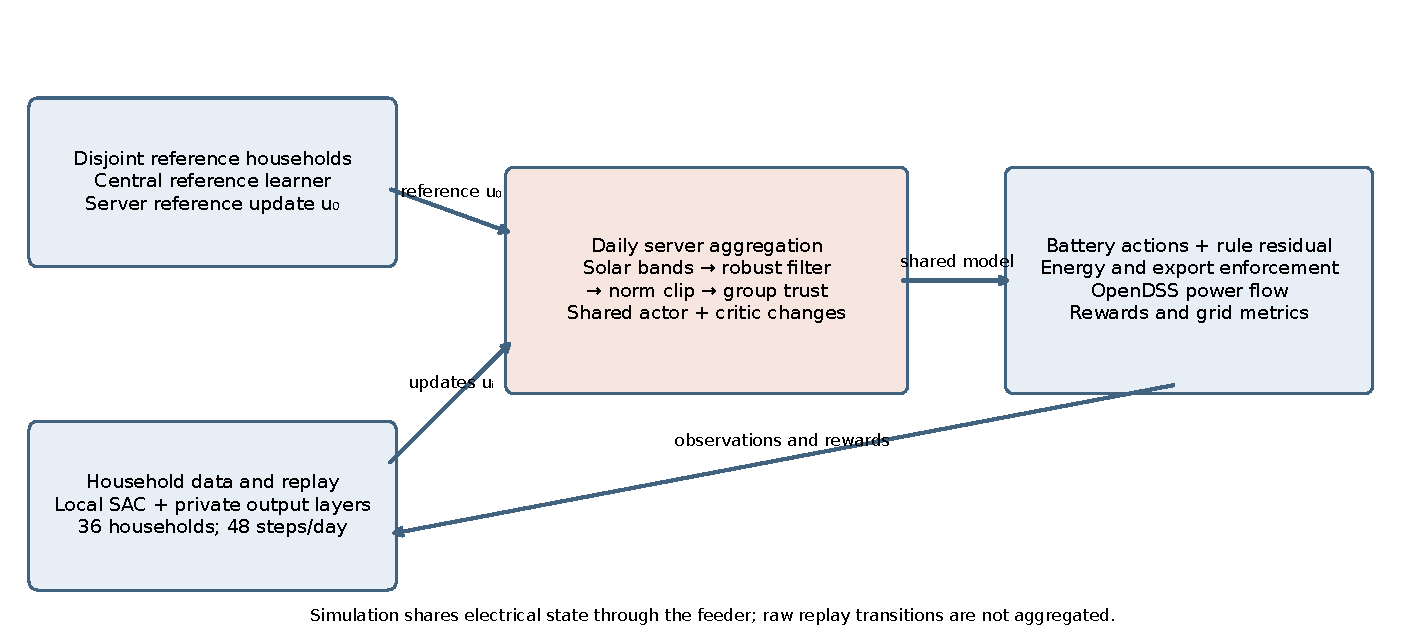
\includegraphics[width=\linewidth]{figures/architecture.pdf}
\caption{Implemented learning and physical-control workflow. Raw replay transitions remain with household learners. The server combines shared parameter changes; a disjoint reference learner provides the trust direction. Export enforcement and power-flow evaluation occur inside the simulator. The reference dataset is an additional trusted resource. Schematic drawn with reproducible Matplotlib code assisted by OpenAI Codex (exact deployed model identifier unavailable).}
\label{fig:architecture}
\end{figure}

% BEGIN SOURCE: tables/configuration.tex
\begin{table}[htbp]
\centering\small
\caption{Implemented configuration for the principal case. Tariffs are fixed experimental inputs; MSL denotes minimum system load.}
\label{tab:configuration}
\resizebox{\linewidth}{!}{%
\begin{tabular}{llll}
\toprule
Parameter & Value & Parameter & Value \\
\midrule
Main/scaling households & 36 / 83 & Time step & 0.5 h \\
Solar scale / cap & 6.6 / 10 kWp & Battery capacity & 3 kWh per kWp \\
Battery power & 5 kW & Round-trip efficiency & 0.90 \\
Source voltage & 1.00 pu; stress 1.02 & Voltage bounds & 216.2--253 V \\
Export cap / ordinary floor & 10 / 1.5 kW & MSL export cap & 0 kW \\
Demand trigger & 3660 MW (scenario) & Voltage margin & 1 V \\
Import: 11:00--16:00 & 0.22680 \$/kWh & Import: 16:00--21:00 & 0.45712 \$/kWh \\
Import: other hours & 0.28035 \$/kWh & Export credit & 0.08660 \$/kWh \\
Daily supply charge & 1.48834 \$/day & Curtailment coefficient & 0.08660 \$/kWh \\
Hidden width / batch & 128 / 128 & Learning rate & 0.0003 \\
Discount / target rate & 0.99 / 0.005 & Warmup & 5 days \\
Training / aggregation & 500 days / daily & Shared payload & 54,400 float32 values \\
Solar bands / robust threshold & 3 / 2.5 & Final clipping bound & 2 median norms \\
\bottomrule
\end{tabular}}
\end{table}

% END SOURCE: tables/configuration.tex


\subsection{Battery operation, household exchange and cost}
For household $i$ at time $t$, let $\ell_{i,t}$ denote load, $s_{i,t}$ available photovoltaic power, $p_{i,t}$ battery power (positive for charging), $q_{i,t}$ curtailed solar power and $e_{i,t}$ stored energy. All power quantities use kW. With $\Delta t=0.5$\,h and one-way efficiency $\eta=\sqrt{0.9}$,
\begin{align}
e_{i,t+1}&=e_{i,t}+\Delta t\left[\eta(p_{i,t})^+-(-p_{i,t})^+/\eta\right],\\
g_{i,t}&=\ell_{i,t}+p_{i,t}-s_{i,t}+q_{i,t},
\end{align}
where $(x)^+=\max(x,0)$ and $g_{i,t}>0$ denotes import. Battery capacity is $E_i=3K_i$\,kWh for solar capacity $K_i$\,kWp, and power rating is $P_i=5$\,kW. Requested power is restricted to
\begin{equation}
-\min(P_i,e_{i,t}\eta/\Delta t)\leq p_{i,t}\leq
\min(P_i,(E_i-e_{i,t})/(\eta\Delta t)).
\end{equation}
Half-hour energy cost is
\begin{equation}
c_{i,t}=\Delta t\left[b_t(g_{i,t})^+-f_t(-g_{i,t})^+\right],
\end{equation}
where $b_t$ and $f_t$ denote import and export prices. Annual bills include the fixed daily supply charge. All experiments use the Ergon 12D 2025--26 schedule, including its 16:00--21:00 peak window. The export price is \$0.0866/kWh, consistent with the Queensland Competition Authority's (QCA) corresponding regional feed-in tariff~\cite{qca}; import prices and the supply charge match the retailer's previous rates from 1 July 2025~\cite{ergontariff}. Table~\ref{tab:configuration} lists these fixed inputs.

\subsection{Export schedules and feeder simulation}
OpenDSS solves an unbalanced constant-power snapshot at each half hour. Household reactive demand corresponds to a power factor of 0.98, while photovoltaic generation and batteries operate at unity power factor. The source voltage is 1.00\,pu in the main experiments and 1.02\,pu in the stress case. Voltage penalties use bounds of 216.2--253\,V.

Each daily export schedule is calculated from the actual load and photovoltaic profiles without batteries. Phase-wise voltage sensitivities are estimated by simultaneously increasing export by 1\,kW at each household on a phase. The half-hour schedule uses the most restrictive voltage headroom on that phase and a 1\,V margin below 253\,V. Outside designated minimum-load periods, household allowances are bounded between 1.5 and 10\,kW. This sensitivity-based construction assumes ideal information; it does not solve an optimal power flow or reproduce an operational utility envelope service.

Minimum system load (MSL) periods are selected when the lowest five-minute Queensland demand within a half hour is below 3660\,MW in the archived 2025 series. Mapping the household calendar to that series preserves the weekday and time of day. The 3660\,MW trigger defines the onerous scenario used for the reported MSL charging outcomes; 2600\,MW is a separate typical reference, not the implemented trigger. Export allowances are set to zero in the selected periods.

When requested export exceeds allowance $L_{i,t}$, the simulator first reduces battery discharge and then curtails any remaining excess solar. This enforces $(-g_{i,t})^+\leq L_{i,t}$ under the implemented assumptions. Voltage exceedances can nevertheless remain because of schedule approximation, phase coupling and the ordinary export floor. Peak transformer apparent power is measured relative to nameplate rating, without a hard loading constraint.

\subsection{Residual SAC control}
The self-consumption rule charges from surplus solar and discharges against household demand from 16:00 to 21:00. The learned action is a residual $a_{i,t}\in[-1,1]$:
\begin{equation}
p^{\mathrm{req}}_{i,t}=P_i\operatorname{clip}\left(a^{\mathrm{rule}}_{i,t}+a_{i,t},-1,1\right).
\end{equation}
Battery-energy and export restrictions convert this requested power into executed power. Initialising the deterministic residual at zero recovers the rule, while stochastic warmup actions explore other schedules.

Soft Actor-Critic (SAC) combines reward and entropy maximisation~\cite{sac,sacapps}. Each household observes eleven features: fractional battery charge; scaled current load and photovoltaic power; price; three tariff-period indicators; sine and cosine of time of day; scaled export allowance; and scaled voltage. The actor outputs a Gaussian mean and log standard deviation. Training uses samples transformed by the hyperbolic tangent; evaluation uses the hyperbolic tangent of the Gaussian mean parameter. The actor and twin critics each have two shared hidden layers of width 128 with rectified linear units and a local output layer. Training uses batch size 128, learning rate $3\times10^{-4}$, discount 0.99 and target interpolation coefficient 0.005.

The local reward is
\begin{equation}
r_{i,t}=-c_{i,t}-0.0866\Delta t\,q_{i,t}
-\Delta t\,h_{i,t}-0.1\,v^{\mathrm{out}}_{i,t},
\end{equation}
where $h_{i,t}$ is excess export power after enforcement and $v^{\mathrm{out}}_{i,t}$ is the voltage deviation outside the prescribed interval, in volts. Successful export enforcement makes the export penalty zero. Rewards are multiplied by ten before SAC updates. Because curtailment is penalised in addition to its effect on the bill, the training objective differs from the reported electricity bill.

Training samples seven-day blocks from the training partition. Stored energy carries between days within a block; a newly sampled block starts half charged, and bootstrapping terminates across that discontinuity. Five days of random-action warmup precede learning. The main experiments use 500 training days, with archived 1000-day runs providing additional clean-learning evidence in Table~\ref{tab:extended_clean}. Validation is performed on day 1 and every 25 training days. Central SAC pools household transitions into one agent, whereas local SAC maintains independent agents and replay buffers. These are comparison architectures, not formal performance bounds.

\subsection{Daily federation and FedGrid}
At the end of each training day, households share the actor and critic hidden-layer parameters while retaining their output layers and replay buffers locally. If $\theta_r$ is the server model at round $r$ and $\theta_{i,r}^{\mathrm{local}}$ the shared part after local training, the update is $u_{i,r}=\theta_{i,r}^{\mathrm{local}}-\theta_r$. The server sets $\theta_{r+1}=\theta_r+\mathcal A(\{u_{i,r}\})$ and copies the shared layers to each household. Target critics, optimiser states and entropy temperatures remain local across broadcasts. The shared vector contains 54,400 float32 values, corresponding to 212.5\,KiB per direction per household, excluding protocol overhead.

For FedGrid, solar capacities determine three quantile bands. Medians of update coordinates, norms, distances and absolute deviations use the lower middle order statistic for even-sized samples, matching the implementation; capacity-band boundaries remain quantiles. Any band with fewer than five received updates is merged with a neighbouring band until sufficiently large or only one remains. In group $g$, define a coordinate median $m_g$ and update distances $d_i=\|u_i-m_g\|_2$. Write $\widetilde d_g=\operatorname{median}_{i\in g}d_i$ and
\begin{equation}
\sigma_g=1.4826\operatorname{median}_{i\in g}|d_i-\widetilde d_g|.
\end{equation}
An update passes when $d_i-\widetilde d_g\leq2.5\max(\sigma_g,1.4826\times10^{-12})$. The stabiliser corresponds to flooring the unscaled median absolute deviation before applying the factor 1.4826, as in the implementation. The rule rejects unusually large distances; it does not reject small distances merely because they differ from the median.

In the final configuration, filtering uses the original updates. Admitted updates are then clipped as
\begin{equation}
\widehat u_i=u_i\min\left(1,\frac{2\operatorname{median}_j\|u_j\|_2}{\max(\|u_i\|_2,10^{-12})}\right),
\end{equation}
where the clipping bound uses all received updates, including filtered ones. If $I_g$ is the admitted subset and $\bar u_g=|I_g|^{-1}\sum_{i\in I_g}\widehat u_i$, the group weight and aggregate are
\begin{equation}
w_g=|I_g|\max(0,\cos(\bar u_g,u_0)),\qquad
\mathcal A=\frac{\sum_gw_g\bar u_g}{\max(\sum_gw_g,10^{-12})}.
\end{equation}
Cosine agreement uses the stabilised implementation: each vector norm is floored at $10^{-8}$ before division, so a zero reference or group mean gives zero agreement. The server reference $u_0$ comes from a central learner using a disjoint set of households, starting its shared layers from the current global model each round. A zero total weight produces a zero aggregate. The original FedGrid clips before filtering at one median norm. Therefore, the final revision changes both operation order and clipping multiplier.

\begin{table}[htbp]
\centering
\caption{FedGrid round procedure, matching the final implementation.}
\label{tab:algorithm}
\begin{tabular}{p{0.94\linewidth}}
\toprule
Receive shared changes and household solar bands; train the disjoint reference learner to obtain $u_0$.\\
Merge small bands; compute robust within-band distances on original changes.\\
Mark distance outliers; compute the clipping bound from all received update norms.\\
Clip admitted changes at twice the median norm and form each admitted group mean.\\
Weight group means by admitted size and nonnegative cosine agreement with $u_0$.\\
Apply the weighted aggregate to shared actor and critic layers; retain local output layers.\\
Log outlier-filter decisions separately from any interpretation of effective weight.\\
\bottomrule
\end{tabular}
\end{table}

\subsection{Bounded update size and effective coefficients}
The clipping and nonnegative group weights imply a deterministic bound on the aggregate norm. Let $B=2\operatorname{median}_j\|u_j\|_2$ and $\epsilon=10^{-12}$. Each clipped update has norm at most $B$, and each group mean therefore also has norm at most $B$. With $W=\sum_gw_g\geq0$, the triangle inequality gives
\begin{equation}
\|\mathcal A\|_2\leq\frac{\sum_gw_g\|\bar u_g\|_2}{\max(W,\epsilon)}
\leq B\frac{W}{\max(W,\epsilon)}\leq B.
\end{equation}
This is a deterministic bound on one shared parameter change, not a guarantee on update direction, learning convergence, household cost or physical safety. In particular, an adversary may still change the direction inside the bounded region.

Conditional on a realised set of group weights, the coefficient on an admitted clipped update is
\begin{equation}
\beta_i=\frac{w_{g(i)}}{|I_{g(i)}|\max(W,\epsilon)},
\end{equation}
with $\beta_i=0$ for filtered updates. Filter admission does not imply $\beta_i>0$: a nonpositive group-reference cosine makes $w_{g(i)}=0$. A positive coefficient also does not prove a nonzero causal effect on the eventual action because weights depend on all updates, vectors can cancel, and later policy dynamics intervene. The distinction between admission and positive coefficients motivates reporting them separately. The identities characterise the realised aggregation rule without establishing Byzantine resilience.

\subsection{Comparators and attack model}
The main comparison comprises FedAvg, median, trimmed mean, Krum, FLTrust, FLAME, original and tuned TAFDRL-style filters, and original and final FedGrid. FedProx is additionally evaluated in clean learning. Trimmed mean and Krum receive the assumed compromised share. FLTrust and FedGrid receive the reference learner; comparators therefore do not all use identical auxiliary information. Table~\ref{tab:comparators} summarises their aggregation and admission semantics.

% BEGIN SOURCE: tables/comparators.tex
\begin{table}[htbp]
\centering\small
\caption{Comparator scope and admission semantics. Source algorithms are adapted to shared SAC parameter changes; original guarantees are not transferred to this setting.}
\label{tab:comparators}
\resizebox{\linewidth}{!}{%
\begin{tabular}{lll}
\toprule
Method & Aggregation principle & Whole-update rejection statistic \\
\midrule
FedAvg / FedProx & Mean / mean with local proximal term & Not defined \\
Median / trimmed mean & Coordinate statistics & Not defined \\
Krum & Select one neighbour-consistent update & Unselected updates \\
FLTrust & Positive cosine trust; norm rescaling & Zero-trust updates \\
FLAME & Majority clustering, clipping and noise & Outside admitted cluster \\
TAFDRL-style & PCA distance and Beta trust & Distance or minimum-trust exclusion \\
FedGrid & Within-band filter and group trust & Filter exclusion; zero-weight groups omitted \\
\bottomrule
\end{tabular}}
\end{table}

% END SOURCE: tables/comparators.tex


Compromised household positions are sampled for each seed and nominal share and remain fixed within a run. A nominal 30\% share selects 11 of 36 homes. Update attacks preserve local training but replace the transmitted changes. The Normalized attacker observes every honest update, queries the aggregation rule and searches fixed grids for directional mixing and magnitude. Adaptation is therefore limited to that search space. Meter poisoning swaps the learner's load and solar observation channels, while the residual self-consumption rule still uses the simulator's true values; reward poisoning reverses local training rewards. Evaluation uses ordinary observations. Separate message-fault experiments drop or delay honest changes by one round.

% BEGIN SOURCE: tables/threats.tex
\begin{table}[htbp]
\centering\small
\caption{Implemented perturbations. Compromised households are fixed within a run; message faults affect honest households.}
\label{tab:threats}
\resizebox{\linewidth}{!}{%
\begin{tabular}{lll}
\toprule
Threat & Perturbation & Knowledge or scope \\
\midrule
Flip & Negate model changes & Own update \\
Scale & Multiply changes by household count & Own update; system size \\
Noise & Gaussian update variance 1000 & Parameter dimension \\
Normalized & Direction and magnitude grid search & All updates; aggregation queries \\
Meter & Swap observed load and solar channels & Local training observations \\
Reward & Reverse local reward sign & Local training rewards \\
Message faults & 10\% drop and 10\% one-round delay & Honest changes; separate scenario \\
\bottomrule
\end{tabular}}
\end{table}

% END SOURCE: tables/threats.tex


The model predictive control (MPC) comparator solves a linear program at midnight using exact daily load, solar, prices and export allowances, with a terminal value for stored energy. It is a daily perfect-foresight reference, not a forecast-based controller or an annual global optimum. The program uses separate nonnegative charge and discharge variables and sends their net power to the simulator. A five-day replay check compares the executed bill with the planned bill; the archived implementation does not apply that consistency check throughout the evaluation horizon. Forecast-based MPC and full-horizon validation of this relaxation remain outside the reported experiments.

% END SOURCE: sections/methods.tex


% BEGIN SOURCE: sections/evaluation.tex
\section{Evaluation design and reporting}
\label{sec:evaluation}
\subsection{Partitions, policy retention and experimental coverage}
Figure~\ref{fig:splits} shows the time partitions, and Table~\ref{tab:coverage} gives the replication for each experimental group. The main attack comparison uses five Ausgrid learning seeds and three ACT retraining seeds. Transfer comparisons involving the original methods use two common seeds, whereas final FedGrid and tuned TAFDRL-style have five available transfer seeds. The archive contains 706 top-level learning logs across groups; these are not independent replicates of a single comparison.

Clean 500-day experiments retain the actor with the lowest validation score. Attack experiments retain the last actor, allowing damage late in training to remain visible rather than selecting an earlier policy. Each attack comparison uses a no-attack last-policy reference from the same aggregation rule. Results from these retention protocols are reported separately.


% BEGIN SOURCE: tables/coverage.tex
\begin{table}[htbp]
\centering\small
\caption{Experimental coverage. The principal Ausgrid, ACT retraining and transfer comparisons contain six attacks and a no-attack reference per method and seed; sensitivity and clean-learning groups have separate designs.}
\label{tab:coverage}
\resizebox{\linewidth}{!}{%
\begin{tabular}{lllll}
\toprule
Setting & Methods & Seeds per method & Households & Policy \\
\midrule
Ausgrid main & 10 & 0--4 (5) & 36 & Last \\
ACT retraining & 10 & 0--2 (3) & 36 & Last \\
ACT transfer, final variants & 2 & 0--4 (5) & 36 & Last \\
ACT transfer, other methods & 8 & 3--4 (2) & 36 & Last \\
Share, fault, scaling, stress & Varies & Mostly 0 (1) & 36 or 83 & Last \\
Clean learning & 4 learned baselines & 0--2 (3) & 36 & Validation-selected \\
\bottomrule
\end{tabular}}
\end{table}

% END SOURCE: tables/coverage.tex


\subsection{Economic damage and household alignment}
All monetary quantities are in Australian dollars (AUD). Let $B_{m,a,s}(H)$ denote annual household-average bill for method $m$, attack $a$, seed $s$ and evaluated positions $H$. Damage is
\begin{equation}
D_{m,a,s}=B_{m,a,s}(H_a)-B_{m,\varnothing,s}(H_a).
\end{equation}
Update attacks use all households in $H_a$, since they corrupt transmitted changes without directly corrupting the physical evaluation. Meter and reward attacks use only the fixed honest positions. Their no-attack references use the same positions, drawing on archived honest-reference runs where necessary. Negative damage is retained and denotes a lower observed bill than the matched reference; it does not imply that an attack improves performance generally.

Ausgrid evaluation covers the full annual period, carrying stored energy between days after an initial half-charge state. ACT evaluation uses 13 separated seven-day blocks, each starting half charged, and annualises energy and cost sums by $365/91$. These are annualised block estimates rather than outcomes from a continuous year. Voltage-exceedance frequency is the proportion of half hours with at least one household above 253\,V; maximum voltage is taken over all evaluated homes and intervals. These frequencies and transformer peaks describe the evaluated intervals and are not annualised as sums.

The reported cycle statistic divides total battery energy throughput by twice the sum of battery capacities. It is a fleet-equivalent cycle measure, or a capacity-weighted average of household equivalent cycles, rather than the arithmetic mean of household cycle counts. Bills and curtailed solar are averaged per household; MSL charging is summed across the street.

For the damage--rejection scatter, the vertical coordinate is
\begin{equation}
W_m=\max_{a\in\mathcal T}\left(\frac{1}{S}\sum_sD_{m,a,s}\right),
\end{equation}
where $\mathcal T$ contains all six attacks. This maximum of attack-wise means differs from the mean of seed-wise maxima. Because the largest mean and its associated attack can change with the seed sample, no confidence interval for the selected maximum is inferred from an individual attack's interval.

\subsection{Recorded rejection and effective contribution}
\label{sec:participation}
The scatter's horizontal coordinate is mean logged honest rejection across the same six attacks and seed scope. For each household, the logged rate is rejected received changes divided by received changes after warmup. Missing legacy entries remain missing, with observation counts retained in the CSV. No-attack rejection is reported separately in the table and heatmap.

Admission decisions have different meanings across methods. FedGrid records within-band outlier rejection; subsequent zero group weight leaves its admitted members recorded as kept. FLTrust records zero-trust updates as rejected. Krum selects one received vector, so most vectors are unselected by design. Median and trimmed mean do not provide a whole-vector admission mask and therefore have no comparable logged rate.

A synthetic diagnostic illustrates the distinction: twelve identical changes opposite to the reference direction pass FedGrid's distance filter, yet produce a zero aggregate. This establishes a property of the statistic, not its prevalence in the energy experiments. Rounded historical rejection logs cannot recover the frequency of zero-weight groups. We therefore distinguish \emph{recorded rejection} from positive aggregation weight and from household fairness.

\subsection{Uncertainty and paired revision analysis}
For a scalar outcome across $S$ seeds, tables report the mean and Student-$t$ 95\% confidence interval half-width,
\begin{equation}
\bar x\ \pm\ t_{0.975,S-1}\,\frac{s_x}{\sqrt S}.
\end{equation}
A single-seed observation is marked $[1]$ without an estimated interval. These small-sample intervals depend on distributional assumptions and are conditional on the fixed household assignment; they do not describe uncertainty across arbitrary networks or household populations.

The revision effect is $D_{\mathrm{final},a,s}-D_{\mathrm{original},a,s}$ on matched seeds, with negative values favouring the final configuration. Transfer pairs use only seeds 3--4 despite the five final-configuration runs. Intervals for these effects are exploratory and unadjusted for multiple comparisons. Overlap of marginal intervals is not interpreted as equivalence.

An exploratory audit applies two-sided exact Wilcoxon signed-rank tests to the five-seed Ausgrid differences, with Holm adjustment within an 18-test robust-comparator family and a six-test original-versus-final family~\cite{scipywilcoxon,holm}. No comparison reaches 0.05 before or after adjustment. The appendix reports the exact p-values and their five-pair resolution limit. These retrospective tests do not complete the larger planned replication study.

\subsection{Artifact construction and verification}
Python scripts derive damage, paired effects and figures from archived logs, exporting the underlying observations and input hashes. Matplotlib renders the figures from those values; no dispatch traces are inferred from aggregate logs. OpenAI Codex assisted with drafting and reproducible analysis and figure scripts; its exact deployed model identifier was unavailable. Assistance with the schematic and partition figures is disclosed in their captions. Source scripts, per-seed values and log hashes support independent verification of the reported calculations.

% END SOURCE: sections/evaluation.tex


% BEGIN SOURCE: sections/selection.tex
\section{Configuration selection and development history}
\label{sec:selection}
\subsection{Time partitions and evaluation exposure}
Ausgrid development uses seven-day blocks from July 2010 to June 2012. Every eighth block, starting at index four, is reserved for validation; the July 2012--June 2013 year is used for evaluation. The residual-controller architecture was also chosen after inspecting evaluation-year bills from earlier controller alternatives, as documented in the archived diagnostics. Those diagnostic runs used earlier implementations and are excluded from the current comparisons. Evaluation outcomes were subsequently inspected before FedGrid was revised. The later numerical selector therefore uses validation scores within a development process already exposed to evaluation outcomes. New learning seeds on the same profiles do not restore an untouched evaluation year.

ACT NextGen uses 52 weeks beginning on 1 January 2018. Every fourth week, starting at index three, is assigned to evaluation, giving 13 weeks. Every eighth week, starting at index one, is assigned to validation, giving seven weeks. The remaining 32 weeks form the training partition. ACT experiments include retraining and transfer without retraining, while retaining the feeder, tariff and battery-control assumptions. The donor audit in the appendix additionally documents imputation across these partition boundaries.

\subsection{Validation criterion}
For each configuration and seed, selection averages the final four validation assessments. Each assessment sums household-average cost and the curtailment penalty across the validation weeks. Validation damage is the attacked score minus the matched no-attack score. Configurations are ranked by the largest attack-wise mean of these paired differences.

FedGrid candidates use flip, scale, noise and Normalized attacks at a nominal 30\% compromised share and seeds 0--2. The tuned TAFDRL-style comparator uses flip and Normalized only. The candidate families consequently have unequal tuning attack sets and search budgets. Their cost-plus-curtailment scores over validation weeks are distinct from the annual evaluation bill damage.

\subsection{Post-hoc rejection constraint}
The robustness-only selector initially chose a configuration applying trust separately to each household. Its worst-case mean validation damage was \$6.2 per household over the validation weeks, and its recorded honest rejection was 30.8\%, compared with 2.0\% for original FedGrid. A numerical eligibility constraint was then added: a FedGrid configuration could reject at most twice the original configuration's recorded honest share, giving a 4.0\% bound for these results. This bound was introduced after the candidate outcomes had been inspected; it was not preregistered. The rejection statistic pools all available nominal-30\% runs for each version: 21 original FedGrid runs (no attack and six attacks across three seeds), 15 runs for a complete FedGrid candidate (no attack and four update attacks), and nine for a tuned TAFDRL-style setting (no attack, flip and Normalized). These are unequal condition pools. The selector rounds its summaries to one decimal before applying the bound and ranking; the historical 4.0\% threshold is twice the rounded original 2.0\%, not a condition-matched rejection comparison. We preserve that historical decision rather than recomputing it with a different pool.

The development record shows that a settings sweep for the household-trust configuration had already finished before the change. The subsequent sweep of the newly selected clipping configuration followed the revised criterion. Thus, the eligibility rule preceded the later sweep, while the earlier settings results were already available.

Under the revised criterion, filtering before clipping with a multiplier of two was selected. Its worst-case validation damage was \$14.5 and recorded honest rejection was 3.4\%. A one-setting-at-a-time sweep considered two or four solar bands and outlier thresholds of 2.0 or 3.0. The default three bands and threshold 2.5 remained selected. The tuned TAFDRL-style filter used $\lambda=2$, minimum trust 0.35 and chi-square level 0.99. Table~\ref{tab:selection_candidates} and Figure~\ref{fig:selection} report the base candidates; Table~\ref{tab:selection_settings} includes both settings sweeps and all four tuned TAFDRL-style choices, with the recorded 40\% FedGrid validation sensitivities.

\subsection{Scope of the final comparison}
The final configurations were frozen after the available evaluation outcomes had been inspected. The present analysis uses that fixed archive, including unfavourable results, without further algorithm changes. Paired effects and exact tests are retrospective analyses of existing runs. The eligibility bound concerns recorded rejection, whose relationship to effective contribution is derived in Section~\ref{sec:methods} and qualified in Section~\ref{sec:participation}.

% END SOURCE: sections/selection.tex


% BEGIN SOURCE: sections/results.tex
\section{Results}
\label{sec:results}
\subsection{Energy management without malicious participants}
In the clean 500-day experiments with validation-selected policies, FedAvg curtails approximately 145\,kWh per household annually, compared with 473\,kWh under the self-consumption rule, a reduction of about 69\%. FedProx and local SAC also reduce curtailment. Across these three learning methods, street-wide charging during designated MSL intervals is approximately 12,400--13,300\,kWh, compared with 1,971\,kWh for the rule. Figure~\ref{fig:energy} and Table~\ref{tab:clean_energy} distinguish these energy outcomes from electricity bills.

Bill differences from the rule are smaller. The rule costs approximately \$953 per household annually; FedAvg, FedProx and local SAC average \$954, \$947 and \$964, respectively, with wide three-seed intervals. Central SAC averages \$879 and perfect-foresight MPC \$591. These references use additional information: central SAC pools household data, and MPC receives exact daily future profiles. The clean results therefore show lower curtailment more clearly than a bill advantage of federation over the rule.

The reduction in curtailment is accompanied by greater battery throughput. FedAvg produces approximately 256 fleet-equivalent cycles annually, compared with 77 for the rule. Because the objective does not monetise this cycling, electricity bills alone do not establish net economic value after degradation and capital costs. These clean outcomes provide the operational context for the attack comparisons. Table~\ref{tab:extended_clean} reports all 1000-day and FedProx-coefficient runs. Mean bills at 1000 days are approximately \$902 for FedAvg, \$890 for FedProx, \$927 for local SAC and \$810 for central SAC; these duration comparisons use validation-selected actors and do not alter the 500-day attack protocol.

\begin{figure}[htbp]
\centering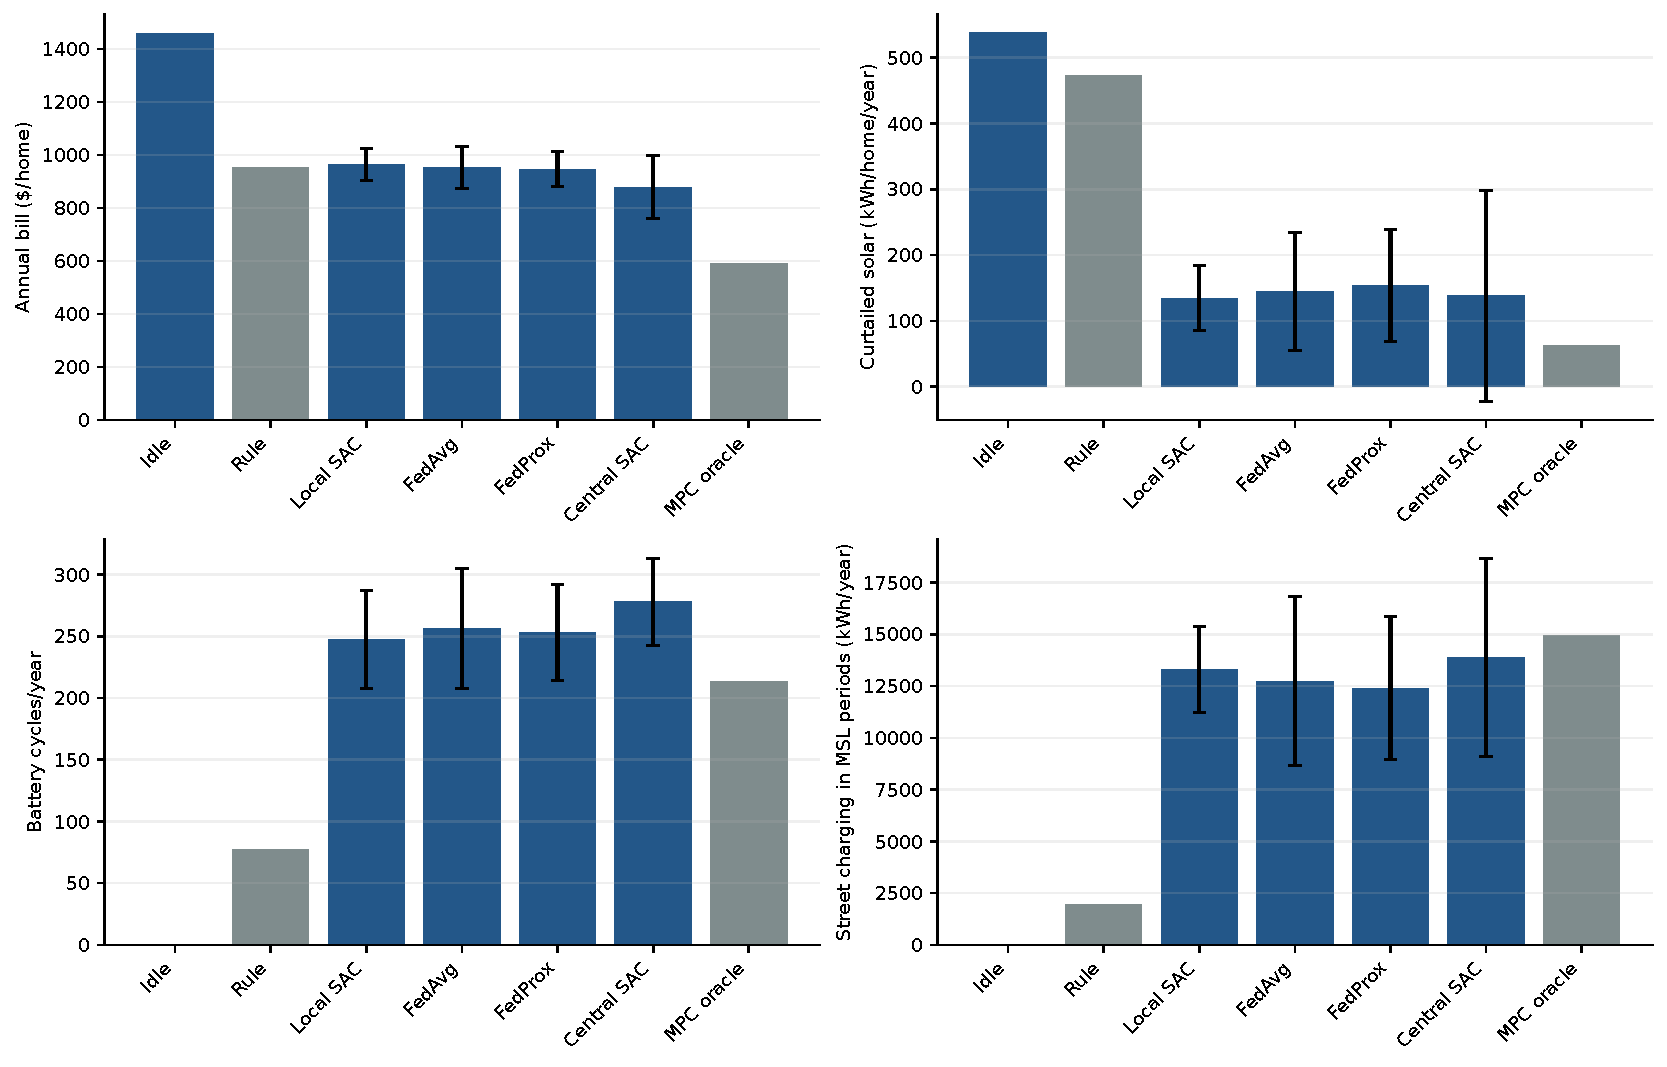
\includegraphics[width=\linewidth]{figures/clean_energy.pdf}
\caption{Clean 500-day energy-management outcomes on Ausgrid. Error bars show Student-$t$ 95\% interval half-widths over three learning seeds. Deterministic baselines have no seed interval. MSL charging is a street total; bill and curtailment are household averages, and cycling is fleet-equivalent. MPC uses perfect daily foresight.}
\label{fig:energy}
\end{figure}

\subsection{Damage under compromised learning contributions}
Table~\ref{tab:ausgrid_damage} reports five-seed Ausgrid damage under all six attacks. FedAvg has mean annual damage of approximately \$532 per household under noise and \$527 under Normalized. Coordinate median and trimmed mean limit some perturbations but retain Normalized damage of approximately \$254 and \$248. Thus, suppressing extreme coordinates does not remove the observed vulnerability to directional poisoning.

Final FedGrid has mean Normalized damage of approximately \$11, compared with \$88 for the original method. Its largest attack-wise mean is approximately \$64 under flip, followed by \$63 under reward poisoning. For comparison, the largest attack-wise means are approximately \$23 for FLTrust, \$50 for FLAME and \$38 for tuned TAFDRL-style. These are descriptive maxima across attacks; the wide seed intervals do not establish a statistical ranking or uniform superiority of final FedGrid.

The final configuration's Normalized estimate has an interval half-width of approximately \$59. Its low mean consequently does not establish immunity, and the comparison remains conditional on the reference data, finite attack search and fixed household assignment.

% BEGIN SOURCE: tables/main_damage.tex
\begin{table}[ht]
\centering\scriptsize
\caption{Ausgrid annual bill damage, seeds 0--4. Entries are mean $\pm$ 95\% confidence interval half-width [seeds], in dollars per household. These are intervals for each attack, not for the maximum across attacks.}
\label{tab:ausgrid_damage}
\resizebox{\linewidth}{!}{%
\begin{tabular}{lrrrrrr}
\toprule
Method & Flip & Scale & Noise & Normalized & Meter & Reward \\
\midrule
FedAvg & 100 $\pm$ 70 [5] & 36 $\pm$ 74 [5] & 532 $\pm$ 92 [5] & 527 $\pm$ 78 [5] & -3 $\pm$ 42 [5] & 42 $\pm$ 46 [5] \\
median & 78 $\pm$ 70 [5] & -8 $\pm$ 28 [5] & -12 $\pm$ 27 [5] & 254 $\pm$ 132 [5] & -10 $\pm$ 11 [5] & 79 $\pm$ 48 [5] \\
trimmed & 64 $\pm$ 27 [5] & -18 $\pm$ 16 [5] & -7 $\pm$ 25 [5] & 248 $\pm$ 77 [5] & -8 $\pm$ 13 [5] & 83 $\pm$ 26 [5] \\
Krum & 41 $\pm$ 99 [5] & 35 $\pm$ 72 [5] & 3 $\pm$ 51 [5] & 47 $\pm$ 98 [5] & 27 $\pm$ 42 [5] & 44 $\pm$ 88 [5] \\
FLTrust & -4 $\pm$ 18 [5] & 4 $\pm$ 4 [5] & -14 $\pm$ 33 [5] & 23 $\pm$ 67 [5] & 19 $\pm$ 6 [5] & 20 $\pm$ 37 [5] \\
FLAME & 50 $\pm$ 58 [5] & 10 $\pm$ 40 [5] & 2 $\pm$ 28 [5] & 43 $\pm$ 55 [5] & 10 $\pm$ 40 [5] & -2 $\pm$ 41 [5] \\
TAFDRL-style & 89 $\pm$ 44 [5] & 14 $\pm$ 16 [5] & -6 $\pm$ 43 [5] & 66 $\pm$ 86 [5] & 15 $\pm$ 22 [5] & 6 $\pm$ 31 [5] \\
TAFDRL-style final & 34 $\pm$ 8 [5] & 21 $\pm$ 25 [5] & -4 $\pm$ 33 [5] & 38 $\pm$ 107 [5] & 6 $\pm$ 26 [5] & 20 $\pm$ 39 [5] \\
FedGrid & 74 $\pm$ 51 [5] & -4 $\pm$ 13 [5] & 47 $\pm$ 24 [5] & 88 $\pm$ 11 [5] & 12 $\pm$ 37 [5] & 48 $\pm$ 53 [5] \\
FedGrid final & 64 $\pm$ 47 [5] & -9 $\pm$ 17 [5] & 19 $\pm$ 34 [5] & 11 $\pm$ 59 [5] & 25 $\pm$ 33 [5] & 63 $\pm$ 56 [5] \\
\bottomrule
\end{tabular}}
\end{table}

% END SOURCE: tables/main_damage.tex

\begin{figure}[htbp]
\centering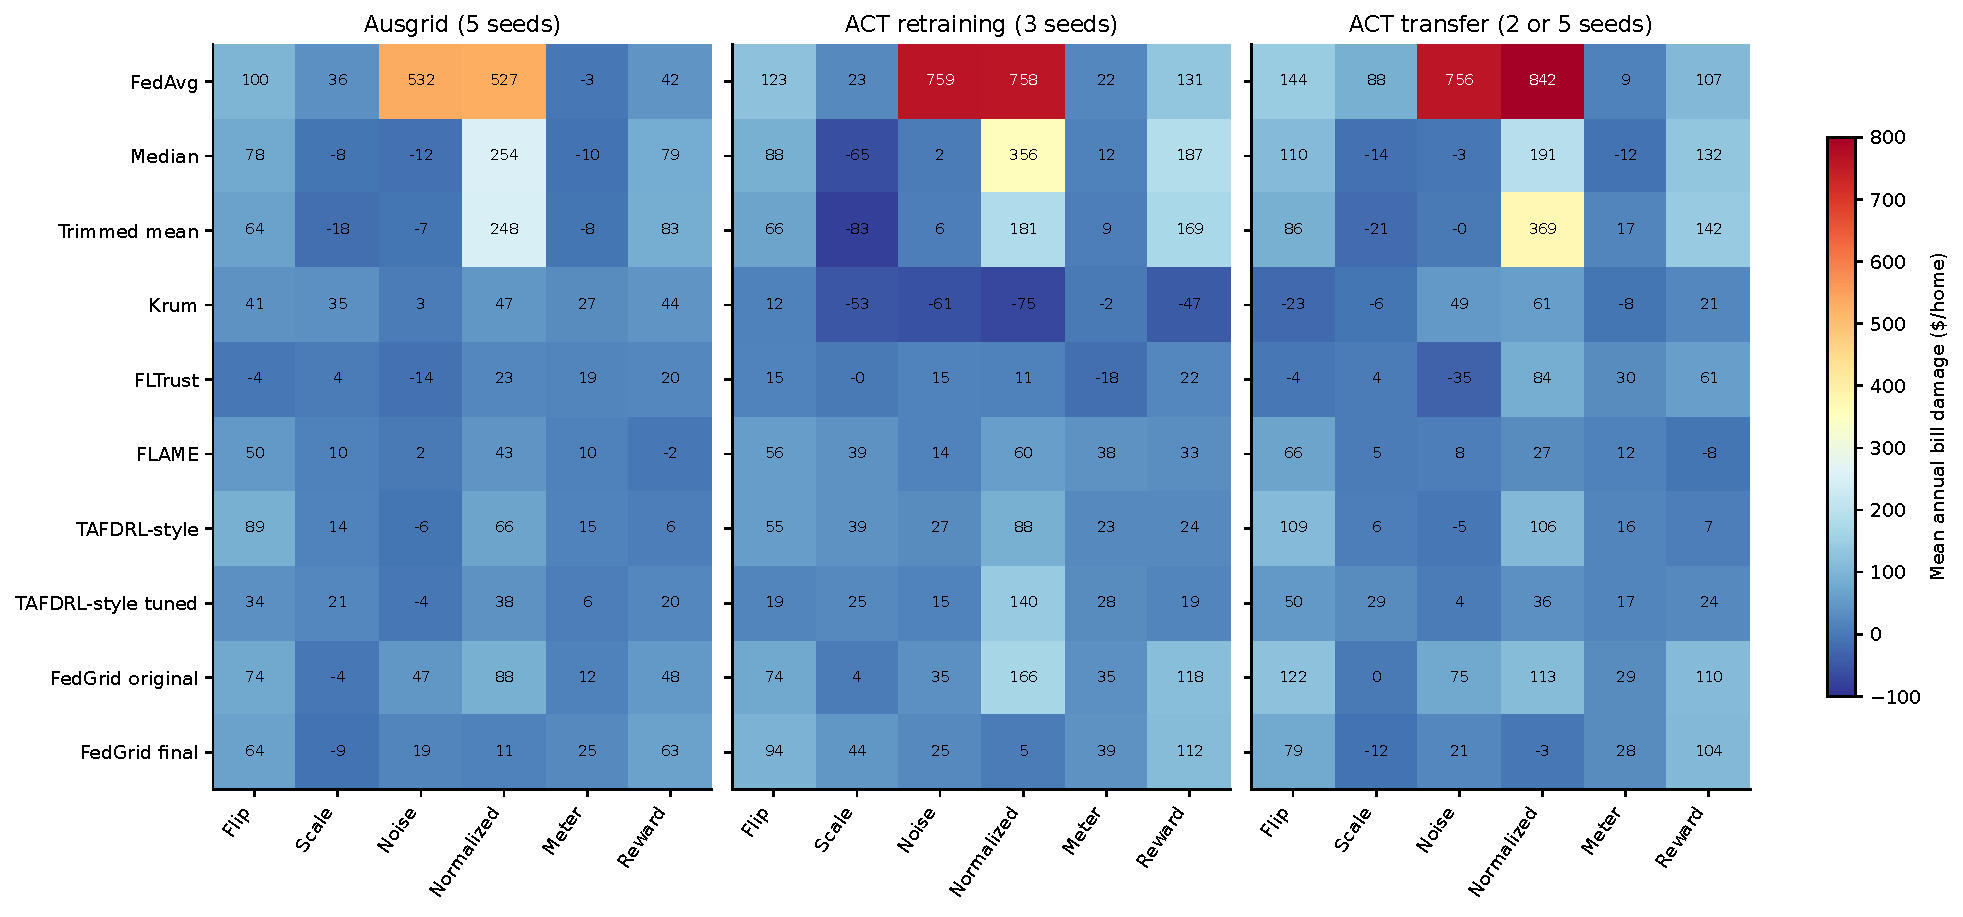
\includegraphics[width=\linewidth]{figures/attack_damage.pdf}
\caption{Mean annual bill damage across six attacks. The same colour scale is used for Ausgrid, ACT retraining and ACT transfer. Transfer uses two seeds for original methods and five for final variants; these unequal means are not paired revision estimates. Update attacks evaluate all homes, while meter and reward attacks evaluate matched honest homes.}
\label{fig:damage}
\end{figure}

\subsection{ACT retraining and transfer}
In three-seed ACT retraining, mean Normalized damage falls from approximately \$166 for original FedGrid to \$5 for the final configuration. Final FedGrid nevertheless incurs approximately \$112 under reward poisoning and \$94 under flip. Table~\ref{tab:act_damage} shows that the attack profile changes with the household data even when feeder and tariff assumptions are retained. These outcomes remain subject to the ACT imputation overlap.


Transfer applies the Ausgrid-trained shared policy and local output layers to ACT households at the corresponding feeder positions without retraining. Final FedGrid has five available seeds; original FedGrid and most comparators have two. The final configuration's five-seed mean Normalized damage is approximately $-\$3$, with an interval half-width of \$60. Reward damage is approximately \$104, with a half-width of \$40, indicating persistent sensitivity to training-time reward corruption. Differences between these unequal method means are not matched revision effects.

\subsection{Matched effect of the FedGrid revision}
Table~\ref{tab:paired_revision} and Figure~\ref{fig:paired} compare final and original FedGrid using matched seeds and attacks. The paired Normalized change in annual damage is $-\$76.8\pm\$67.5$ on Ausgrid and $-\$160.6\pm\$97.5$ on ACT. The descriptive Student-$t$ intervals exclude zero, but the five-pair Ausgrid exact test gives $p=0.0625$ and $p_{\mathrm{Holm}}=0.375$ within the six-attack revision family. We report the estimated reduction without a multiplicity-controlled improvement claim. Transfer gives $-\$74.1\pm\$175.9$ on the two common seeds, demonstrating the limited precision of the matched estimate.

The revision does not lower every observed attack mean. ACT scale damage changes by approximately +\$40, and Ausgrid meter damage by approximately +\$14. Their broad intervals do not establish systematic deterioration; they nevertheless qualify an interpretation based only on the favourable Normalized result.

\begin{figure}[htbp]
\centering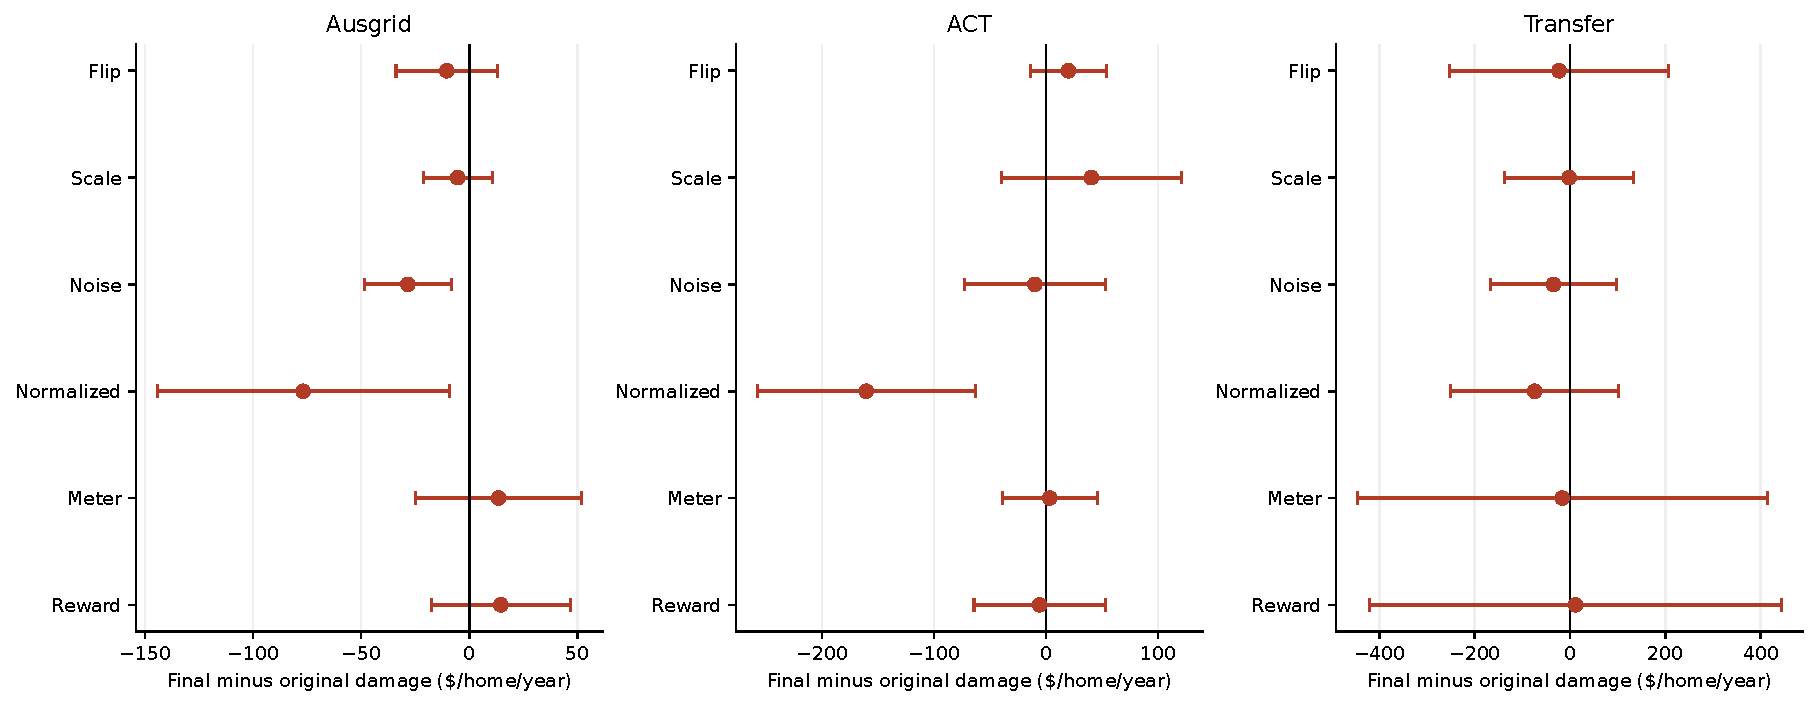
\includegraphics[width=\linewidth]{figures/paired_revision.pdf}
\caption{Matched final-minus-original change in annual attack damage. Negative values favour the revision. Error bars are unadjusted 95\% Student-$t$ intervals over five Ausgrid, three ACT or two common transfer seeds. The horizontal scales vary to display the substantially greater transfer uncertainty.}
\label{fig:paired}
\end{figure}

\subsection{Recorded rejection and the apparent trade-off}
Figure~\ref{fig:tradeoff} plots the largest attack-wise mean bill damage against mean logged honest rejection, with matching seed scopes within each panel. Final FedGrid records fewer rejected honest vectors than several comparators and lower noise and Normalized damage than FedAvg. FedAvg, median and trimmed mean are omitted from the scatter because their logs provide no comparable whole-vector rejection rate.

The horizontal coordinate has method-specific admission semantics and omits zero-weight FedGrid groups. The scatter therefore describes logged behaviour rather than a common participation frontier. Lower rejection does not establish that more households contribute positive weight, and the same qualification applies to the post-hoc eligibility bound.

Table~\ref{tab:rejection} and Figure~\ref{fig:rejection} retain attack-specific rates, observation counts and no-attack references. Krum's high rate reflects its single-vector selection rule. Some older Krum logs lack rejection statistics; summaries use the available observations without reconstructing missing histories.
\begin{figure}[htbp]
\centering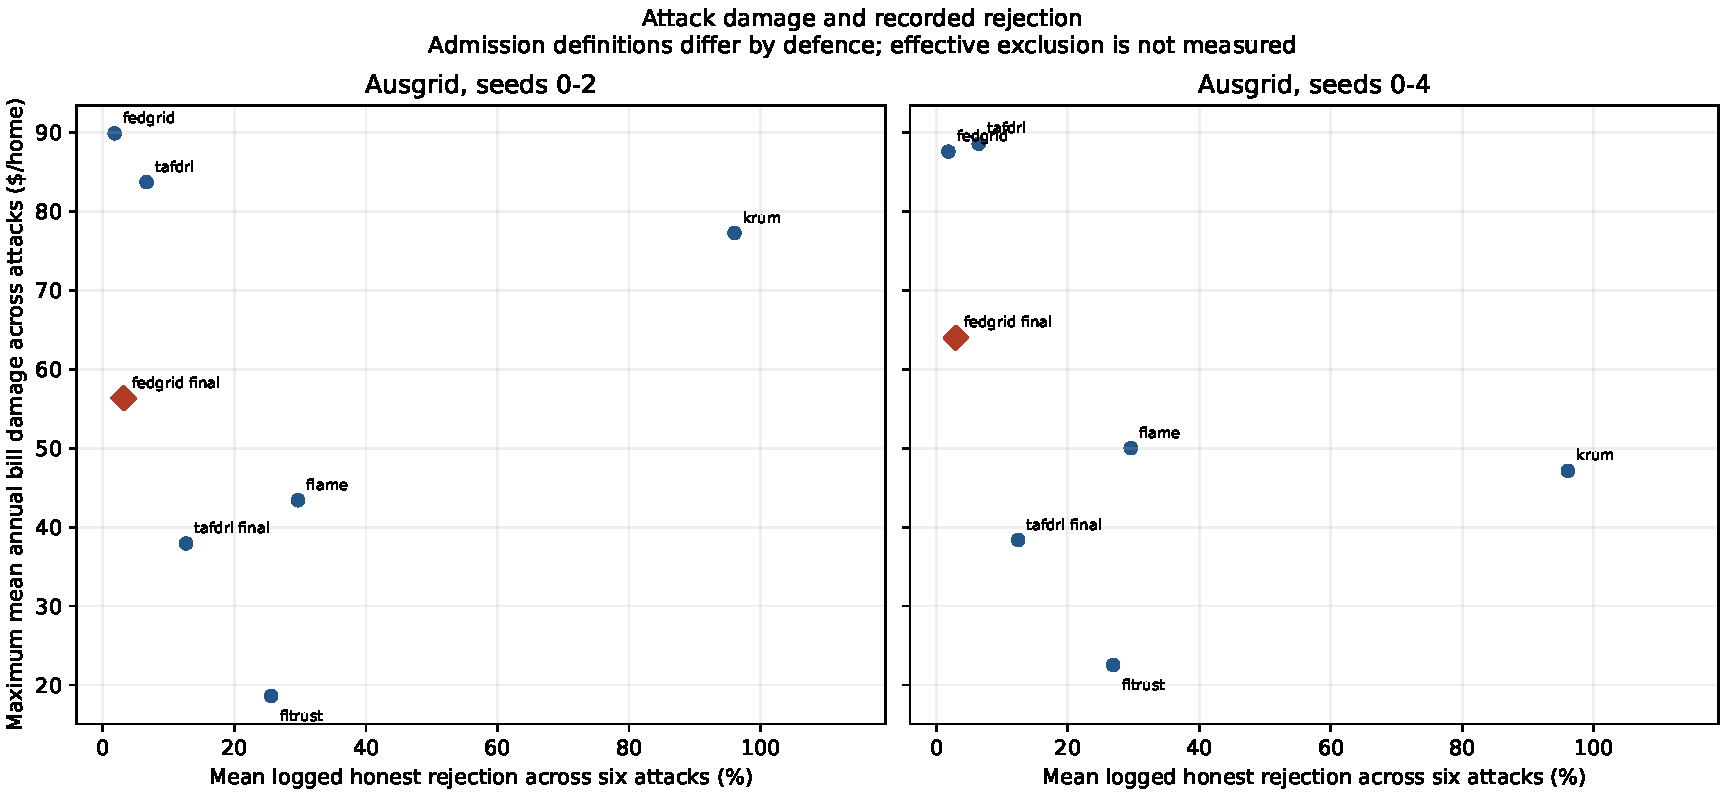
\includegraphics[width=\linewidth]{figures/damage_rejection.pdf}
\caption{Worst-case mean annual bill damage against mean logged honest rejection over the six attacks, at nominal 30\% compromise. Panels use seeds 0--2 and 0--4. Rejection definitions differ across methods and omit zero-weight groups for FedGrid. The vertical coordinate is the maximum of attack means, without an asserted confidence interval for that maximum.}
\label{fig:tradeoff}
\end{figure}

\begin{figure}[htbp]
\centering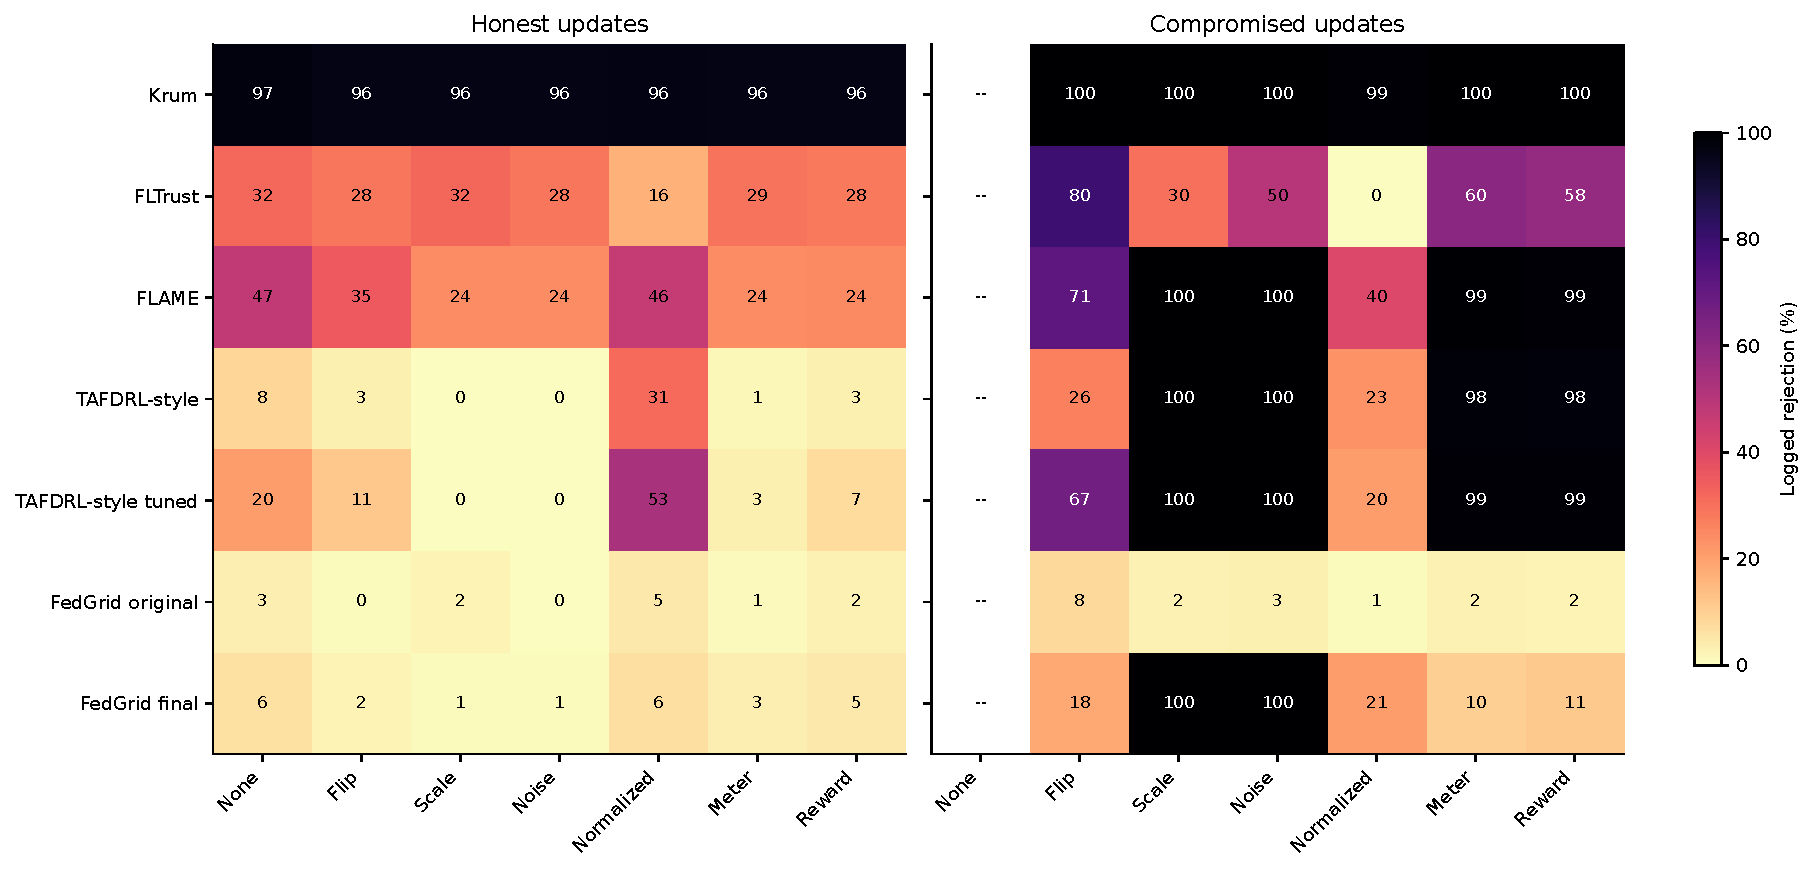
\includegraphics[width=\linewidth]{figures/rejection_heatmap.pdf}
\caption{Mean logged rejection of honest and compromised updates on Ausgrid, seeds 0--4 where available. Dashes indicate unavailable statistics, including compromised rejection in no-attack runs. The values describe method-specific admission decisions, not a uniformly defined exclusion event.}
\label{fig:rejection}
\end{figure}

\subsection{Electrical outcomes and observed violations}
Table~\ref{tab:electrical} reports voltage and transformer outcomes for the no-attack last-policy references, and Figure~\ref{fig:electrical} compares transformer peaks. Each run contributes its peak over the evaluated intervals; the displayed mean and interval summarise those run-level peaks. They do not bound loading in other conditions. These electrical outcomes complement bill damage because simultaneous charging can alter feeder loading even when household costs remain low.



Small voltage-exceedance rates are present in the no-attack logs and are retained at three-decimal precision in Table~\ref{tab:electrical}. Final FedGrid's five-seed mean is $0.010\pm0.028\%$, calculated from the logged rounded rates; its seed-4 run records 0.05\% exceedance and a maximum of 253.60\,V. Averaging run maxima does not make that individual violation disappear.

Attack-time physical outcomes also matter. Table~\ref{tab:attack_electrical} reports maxima over every principal attack run. Under Normalized poisoning, FedAvg reaches transformer peaks of 108.89\% and 113.84\% in seeds 1 and 4. In the single-seed 1.02\,pu final FedGrid no-attack case, the recorded voltage-exceedance rate is 0.27\% and maximum voltage is 254.09\,V. These observations demonstrate why enforced export allowances must be distinguished from voltage and transformer guarantees.

% END SOURCE: sections/results.tex


% BEGIN SOURCE: sections/discussion.tex
\section{Discussion}
\label{sec:discussion}
\subsection{What the revision establishes}
The largest observed improvement of final FedGrid concerns the Normalized attack. Matched estimates have the same direction on Ausgrid and ACT, while transfer remains imprecise. The ablations suggest that clipping before filtering can obscure magnitude differences relevant to outlier detection. However, the final configuration changes both filter order and clipping bound. The existing comparisons therefore characterise the combined revision without isolating either change as its cause.

The same distinction applies to grouping and trust. Capacity bands are intended to accommodate legitimate household differences, but their presence does not demonstrate fair treatment, and the ablations do not establish that grouping independently produces low rejection. Reference trust can suppress an adverse direction while assigning zero weight to an entire admitted group. The mechanism analysis thus supports a precise account of the aggregation rule without proving that each component independently benefits participation or robustness.

\subsection{Participation as a measurable operational outcome}
Participation has at least three observable stages: reception of an update, passage through the outlier filter and assignment of positive aggregation weight. Reliable communication does not ensure admission, and admission does not ensure positive weight. Even a positive coefficient may have little effect on the resulting policy because contributions interact and can cancel.

Historical logs capture only part of this process. They identify recorded filter decisions and aggregate bills, but not a household-level financial effect of exclusion. A corresponding economic analysis would compare the same household and seed under an averaging reference and each defence, alongside contribution rates and solar-capacity strata. These measurements would connect the aggregation decisions to household outcomes; the current rejection summaries do not establish that connection. The rounded per-home logs nevertheless permit a filter-level stratification (Table~\ref{tab:heterogeneity}): under Normalized attack, final FedGrid records approximately 9.8\% rejection for homes at the unusual solar-capacity thresholds and 4.1\% for other honest homes. These conditional logged rates do not measure effective influence.

\subsection{Energy value and physical protection}
The clean experiments show lower curtailment and greater charging during the designated MSL periods more clearly than reduced bills. This pattern is consistent with the training objective, which penalises curtailment in addition to direct cost. It also involves higher battery throughput without an explicit replacement or degradation charge. Consequently, improved solar absorption cannot be interpreted as a complete economic benefit from the electricity bill alone.

Physical protection also depends on the surrounding control system. Export compliance is enforced by simulator action correction, while transformer loading is measured and the envelope schedule approximates voltage constraints. The ACT perfect-foresight MPC reference reaches approximately 110\% peak transformer loading, and the higher-voltage baseline exhibits voltage violations. Cost, export compliance and network loading therefore require separate reporting; satisfying the implemented envelope does not imply that every electrical limit is satisfied.

\subsection{Implications for an implementable controller}
The archived single-core laptop benchmark measures decision times of 0.04--0.06\,ms for one household and approximately 353--356\,MiB peak process memory. The memory unit reflects the Linux benchmark's conversion of resident-set size. These observations establish the measured software's performance on that machine, rather than Raspberry Pi or inverter-controller feasibility. They also exclude the reference learner, server aggregation, communications, recovery and secure transport.

Forecast-based receding-horizon control, reference-household mismatch and explicit contribution logging remain important comparisons. The current perfect-foresight reference and ideal-information envelopes leave their effects unresolved. Evaluating those conditions would determine how much of the observed protection and energy performance persists under implementable information and computing constraints.

% END SOURCE: sections/discussion.tex


% BEGIN SOURCE: sections/limitations.tex
\section{Limitations}
\label{sec:limitations}
\paragraph{Development and selection.}
The Ausgrid evaluation year informed earlier residual-controller choices and was inspected before the aggregation revision, and the numerical rejection bound was added after candidate results and an earlier household-trust sweep were available. Selection from validation scores therefore occurred within an evaluation-exposed development process. Further seeds on the same profiles do not supply a new chronological holdout; no prospective registration is claimed.

\paragraph{Effective participation.}
Rejection statistics have method-specific definitions, are rounded and are missing from some legacy logs. They omit admitted FedGrid groups with zero weight. These records cannot reconstruct a common false-positive rate or equitable household influence, and individual costs associated with exclusion have not been measured. The historical eligibility rule also pools different attack conditions for the original method and candidate versions.

\paragraph{Data processing and generalisation.}
Monthly irradiance ratios rescale historical Ausgrid solar without a full location-specific physical model. ACT retains Canberra profiles under the same simulated feeder and Queensland tariff, and imputation can use future days and cross weekly partitions. It is consequently not a strictly isolated external holdout. Reinitialising separated evaluation weeks at half charge also affects energy accounting. The experiments do not sample a broad population of independent feeders.

\paragraph{Information and physical assumptions.}
Export schedules use actual daily profiles, reference data are assumed trustworthy and available, and MPC uses perfect daily foresight. Approximate voltage sensitivity and measured rather than constrained transformer loading leave some physical requirements unenforced. The MPC linear program also permits simultaneous charge and discharge, whereas replay executes their net power; the five-day consistency check does not validate that relaxation across the full horizon. Monetary ageing, uncertain inverter response, communication security and field calibration are omitted. Retaining raw records locally does not provide differential privacy or protection from inference through model updates.

\paragraph{Comparator fidelity and threat coverage.}
TAFDRL-style is a reconstruction, FLAME is adapted from a backdoor setting, and the Normalized attacker uses a finite search differing from the source procedure. Methods also have unequal auxiliary information and tuning attack sets. Results therefore concern the implemented configurations, without a general resilience theorem for their learning-control dynamics.

\paragraph{Statistical scope.}
Principal comparisons use three or five seeds, and many sensitivities use one. Intervals are conditional on fixed household assignment and preprocessing, and paired revision intervals are exploratory and unadjusted. A maximum selected across attacks needs its own uncertainty analysis. Exact five-seed tests do not reject after family-wise adjustment; this does not establish equivalence. The expanded replication, forecast-based MPC and individual bill analyses remain uncompleted.

% END SOURCE: sections/limitations.tex


% BEGIN SOURCE: sections/conclusion.tex
\section{Conclusion}
FedGrid combines solar-capacity grouping, robust filtering, clipping and reference-based weighting for federated battery control. In the five-seed Ausgrid archive, the final configuration, which changes filter order and clipping strength, reduces observed mean annual Normalized-attack damage from approximately \$88 to \$11 per household. ACT retraining shows a reduction in the same direction, subject to preprocessing overlap. The exact five-seed signed-rank comparisons do not establish a difference at the 0.05 level, and reward poisoning remains a weakness.

The evaluation separates economic protection from energy utilisation and admission behaviour. Clean FedAvg substantially reduces curtailment relative to the rule, while bill differences are modest and battery throughput increases. Filter admission does not ensure positive aggregation weight, just as a bound on aggregate norm does not guarantee a favourable direction or safe controller behaviour.

These findings support evaluating federated energy control through attack-specific bill damage, electrical outcomes and realised contribution weights. Partition-isolated preprocessing, independent evaluation, matched information assumptions and household-level cost accounting would strengthen the evidence connecting aggregation decisions to reliable and economically useful collaboration.

% END SOURCE: sections/conclusion.tex


% BEGIN SOURCE: sections/declarations.tex
\section*{Declarations}
\paragraph{Data and code availability.}
The accompanying computational artifacts include analysis scripts, numerical figure data, per-seed comparisons and input-log hashes. Public archival identifiers and release terms have not been assigned.
\paragraph{Funding, competing interests and author contributions.}
\textit{Author statements pending confirmation.}
\paragraph{Declaration of generative AI and AI-assisted technologies in manuscript preparation.}
OpenAI Codex assisted with drafting, source checking, analysis scripts and reproducible figure construction. The exact deployed model identifier was unavailable. Figures derive from the recorded data through the supplied workflows. The text and computational artifacts remain subject to human author verification and approval.

% END SOURCE: sections/declarations.tex

\clearpage

% BEGIN SOURCE: references.tex
\begin{thebibliography}{99}
\bibitem{fedavg} B. McMahan, E. Moore, D. Ramage, S. Hampson and B. A. y Arcas, ``Communication-Efficient Learning of Deep Networks from Decentralized Data,'' in \emph{AISTATS}, PMLR 54, pp. 1273--1282, 2017. \url{https://proceedings.mlr.press/v54/mcmahan17a.html}.
\bibitem{fedprox} T. Li, A. K. Sahu, M. Zaheer, M. Sanjabi, A. Talwalkar and V. Smith, ``Federated Optimization in Heterogeneous Networks,'' \emph{Proceedings of Machine Learning and Systems}, vol. 2, 2020. \url{https://proceedings.mlsys.org/paper_files/paper/2020/hash/1f5fe83998a09396ebe6477d9475ba0c-Abstract.html}.
\bibitem{sac} T. Haarnoja, A. Zhou, P. Abbeel and S. Levine, ``Soft Actor-Critic: Off-Policy Maximum Entropy Deep Reinforcement Learning with a Stochastic Actor,'' in \emph{ICML}, PMLR 80, pp. 1861--1870, 2018. \url{https://proceedings.mlr.press/v80/haarnoja18b.html}.
\bibitem{sacapps} T. Haarnoja et al., ``Soft Actor-Critic Algorithms and Applications,'' arXiv:1812.05905, 2018. \url{https://arxiv.org/abs/1812.05905}.
\bibitem{sievers} J. Sievers, P. Henrich, M. Beichter, R. Mikut, V. Hagenmeyer, T. Blank and F. Simon, ``Federated reinforcement learning for sustainable and cost-efficient energy management,'' \emph{Energy and AI}, vol. 21, article 100521, 2025. \url{https://doi.org/10.1016/j.egyai.2025.100521}.
\bibitem{krum} P. Blanchard, E. M. El Mhamdi, R. Guerraoui and J. Stainer, ``Machine Learning with Adversaries: Byzantine Tolerant Gradient Descent,'' in \emph{Advances in Neural Information Processing Systems}, 2017. \url{https://papers.nips.cc/paper/6617-machine-learning-with-adversaries-byzantine-tolerant-gradient-descent.pdf}.
\bibitem{yin} D. Yin, Y. Chen, R. Kannan and P. Bartlett, ``Byzantine-Robust Distributed Learning: Towards Optimal Statistical Rates,'' in \emph{ICML}, PMLR 80, pp. 5650--5659, 2018. \url{https://proceedings.mlr.press/v80/yin18a.html}.
\bibitem{fltrust} X. Cao, M. Fang, J. Liu and N. Z. Gong, ``FLTrust: Byzantine-robust Federated Learning via Trust Bootstrapping,'' in \emph{NDSS}, 2021. \url{https://doi.org/10.14722/ndss.2021.24434}.
\bibitem{flame} T. D. Nguyen et al., ``FLAME: Taming Backdoors in Federated Learning,'' in \emph{31st USENIX Security Symposium}, pp. 1415--1432, 2022. \url{https://www.usenix.org/conference/usenixsecurity22/presentation/nguyen}.
\bibitem{fang} M. Fang, X. Wang and N. Z. Gong, ``Provably Robust Federated Reinforcement Learning,'' in \emph{The ACM Web Conference}, pp. 896--909, 2025. \url{https://doi.org/10.1145/3696410.3714728}. Author manuscript: \url{https://arxiv.org/abs/2502.08123}.
\bibitem{tafdrl} R. Sepehrzad, H. Hosseinalibeiki, N. Taghinezhad, N. Khosravi, A. Al Durra and M. S. Sadabadi, ``Enhanced cyber-resilience in flexible energy markets for microgrids: A trust-aware federated deep reinforcement learning framework,'' \emph{Applied Energy}, vol. 406, article 127282, 2026. \url{https://doi.org/10.1016/j.apenergy.2025.127282}.
\bibitem{ausgrid} E. L. Ratnam, S. R. Weller, C. M. Kellett and A. T. Murray, ``Residential load and rooftop PV generation: an Australian distribution network dataset,'' \emph{International Journal of Sustainable Energy}, vol. 36, no. 8, pp. 787--806, 2017. \url{https://doi.org/10.1080/14786451.2015.1100196}.
\bibitem{nextgen} B. Sturmberg and M. Shaw, \emph{Select data from the NextGen energy storage trial in the ACT, Australia}, version 1, Zenodo, 2025. \url{https://doi.org/10.5281/zenodo.14885589}.
\bibitem{csiro} F. Geth, T. Brinsmead, S. West, P. Goldthorpe, B. Spak, G. Cross and J. Braslavsky, \emph{National Low-Voltage Feeder Taxonomy Study}, CSIRO, Newcastle, 2021. \url{https://doi.org/10.25919/2tas-7213}. OpenDSS models: \url{https://github.com/csiro-energy-systems/RepresentativeLVNetworks}.
\bibitem{energex} Energex, ``About Dynamic Connections,'' official service information, accessed 11 November 2026. \url{https://www.energex.com.au/our-services/connections/residential-and-commercial-connections/solar-connections-and-other-technologies/dynamic-connections-for-energy-exports/about-dynamic-connections}.
\bibitem{qca} Queensland Competition Authority, \emph{Solar feed-in tariff 2025--26: Final determination}, 2025. \url{https://www.qca.org.au/wp-content/uploads/2024/12/final-determination-solar-fit-2025-26-post-board20460672.pdf}.

\bibitem{ergontariff} Ergon Energy Retail, ``Residential tariffs: previous rates from 1 July 2025,'' official tariff schedule, accessed 11 November 2026. \url{https://www.ergon.com.au/retail/residential/tariffs-and-prices/residential-tariffs}.
\bibitem{scipywilcoxon} SciPy contributors, ``scipy.stats.wilcoxon,'' official API reference. The computations use the installed SciPy version recorded with the artifacts. \url{https://docs.scipy.org/doc/scipy/reference/generated/scipy.stats.wilcoxon.html}.
\bibitem{holm} S. Holm, ``A Simple Sequentially Rejective Multiple Test Procedure,'' \emph{Scandinavian Journal of Statistics}, vol. 6, no. 2, pp. 65--70, 1979. \url{https://www.jstor.org/stable/4615733}.
\end{thebibliography}

% END SOURCE: references.tex

\clearpage

% BEGIN SOURCE: sections/appendix.tex
\appendix
\setcounter{figure}{0}
\setcounter{table}{0}
\renewcommand{\theHfigure}{appendix.\arabic{figure}}
\renewcommand{\theHtable}{appendix.\arabic{table}}
\section{Extended evaluation and reproducibility}
\label{sec:appendix}
The appendix provides detailed outcomes, sensitivity cases and audits of the fixed experiment archive. Plotting scripts export the underlying observations as CSV and identify input logs by SHA-256 hashes. These calculations analyse existing runs without retraining controllers or replacing outcomes. Replication and single-seed cases are distinguished throughout.

\subsection{Detailed tabulations and development displays}
Tables and figures in this subsection give the development criteria, data partitions and numerical outcomes corresponding to the principal comparisons.

% BEGIN SOURCE: tables/selection_candidates.tex
\begin{table}[htbp]
\centering\small
\caption{Development-set selection of FedGrid variants. Damage is in dollars over the validation weeks and uses a bill-plus-curtailment score. The post-hoc 4.0\% bound uses the rounded original rejection rate. Rejection pools differ: 21 original runs versus 15 per complete candidate. The last column is the mean of per-run maximum honest-household rejection, not the maximum across runs.}
\label{tab:selection_candidates}
\resizebox{\linewidth}{!}{%
\begin{tabular}{llll}
\toprule
Variant & Worst validation damage & Honest rejection (\%) & Mean run maximum (\%) \\
\midrule
original & 26.0 & 2.0 & 18.0 \\
filter\_first & 19.0 & 3.8 & 28.2 \\
filter\_first\_clip2 & 14.5 & 3.4 & 27.3 \\
filter\_first\_guard & 21.2 & 6.7 & 27.6 \\
filter\_first\_home\_trust & 6.2 & 30.8 & 70.6 \\
without\_clip & 15.3 & 3.5 & 29.4 \\
\bottomrule
\end{tabular}}
\end{table}

% END SOURCE: tables/selection_candidates.tex


\begin{figure}[htbp]
\centering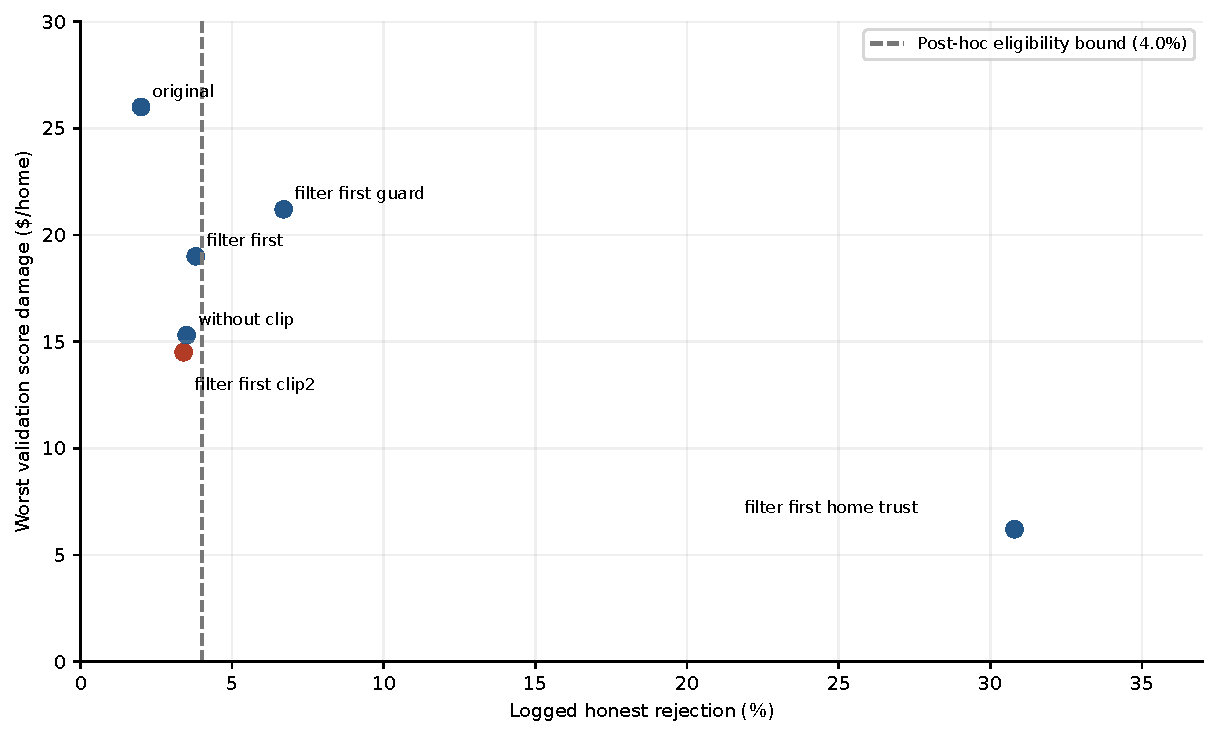
\includegraphics[width=.9\linewidth]{figures/selection_candidates.pdf}
\caption{Candidate selection on validation data, seeds 0--2. The dashed rejection bound was introduced after inspecting candidate results. Validation damage uses a bill-plus-curtailment score over validation weeks; it is not annual evaluation bill damage.}
\label{fig:selection}
\end{figure}

\begin{figure}[htbp]
\centering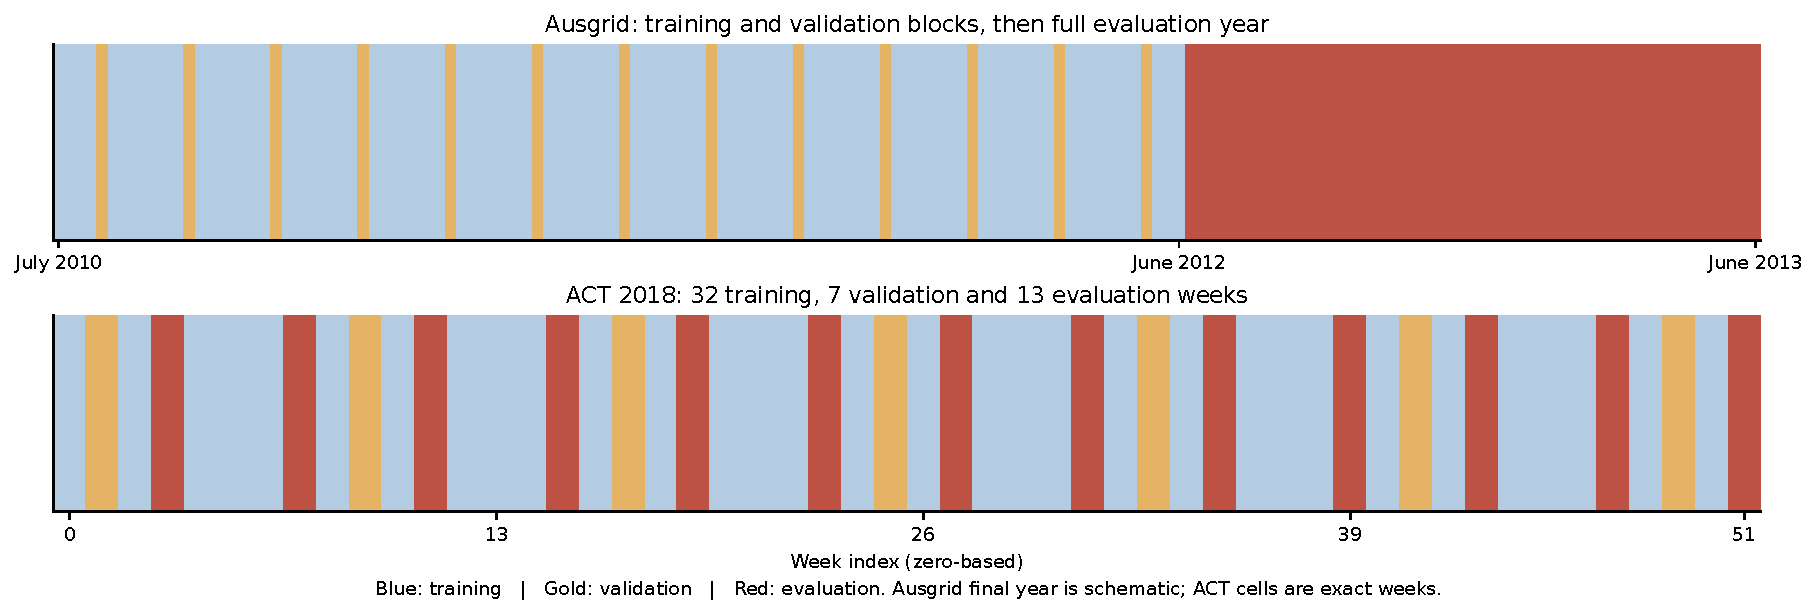
\includegraphics[width=\linewidth]{figures/data_splits.pdf}
\caption{Ausgrid and ACT partitions. The Ausgrid evaluation year is shown schematically after the 104 seven-day development blocks. ACT cells show the exact interleaved weekly assignment. New learning seeds do not create a new chronological holdout. Diagram code was assisted by OpenAI Codex (exact deployed model identifier unavailable).}
\label{fig:splits}
\end{figure}


% BEGIN SOURCE: tables/clean_energy.tex
\begin{table}[htbp]
\centering\small
\caption{Clean 500-day learning with validation-selected policies, Ausgrid. Mean $\pm$ 95\% interval half-width [seeds]; deterministic baselines have one observation. MSL charging is a street-wide total; bills and curtailment are household averages. Cycles are total throughput divided by twice total fleet capacity.}
\label{tab:clean_energy}
\resizebox{\linewidth}{!}{%
\begin{tabular}{lllll}
\toprule
Method & Bill (\$/yr) & Curtailment (kWh/yr) & Cycles/yr & MSL charge (kWh) \\
\midrule
Idle & 1457.8 [1] & 537.7 [1] & 0.0 [1] & 0.0 [1] \\
Rule & 953.0 [1] & 473.2 [1] & 77.5 [1] & 1971.1 [1] \\
Local SAC & 963.8 $\pm$ 61.2 [3] & 134.8 $\pm$ 49.4 [3] & 247.4 $\pm$ 39.4 [3] & 13307.6 $\pm$ 2085.6 [3] \\
FedAvg & 954.3 $\pm$ 79.0 [3] & 144.6 $\pm$ 89.9 [3] & 255.9 $\pm$ 48.6 [3] & 12735.2 $\pm$ 4074.3 [3] \\
FedProx & 947.3 $\pm$ 65.2 [3] & 153.5 $\pm$ 84.8 [3] & 252.7 $\pm$ 38.8 [3] & 12396.6 $\pm$ 3452.8 [3] \\
Central SAC & 879.1 $\pm$ 117.7 [3] & 137.9 $\pm$ 160.3 [3] & 277.7 $\pm$ 34.9 [3] & 13872.7 $\pm$ 4775.5 [3] \\
MPC oracle & 591.0 [1] & 62.9 [1] & 213.4 [1] & 14942.1 [1] \\
\bottomrule
\end{tabular}}
\end{table}

% END SOURCE: tables/clean_energy.tex



% BEGIN SOURCE: tables/act_damage.tex
\begin{table}[htbp]
\centering\small
\caption{Annual bill damage on ACT. Mean $\pm$ 95\% interval half-width [seeds], dollars per household. Transfer coverage differs by method.}
\label{tab:act_damage}
\resizebox{\linewidth}{!}{%
\begin{tabular}{lllllll}
\toprule
Method & Flip & Scale & Noise & Normalized & Meter & Reward \\
\midrule
FedAvg & 123.1 $\pm$ 89.9 [3] & 23.5 $\pm$ 151.6 [3] & 758.9 $\pm$ 123.1 [3] & 757.7 $\pm$ 384.8 [3] & 21.7 $\pm$ 165.9 [3] & 131.4 $\pm$ 138.9 [3] \\
Median & 87.8 $\pm$ 169.2 [3] & -64.6 $\pm$ 47.8 [3] & 2.3 $\pm$ 177.8 [3] & 356.4 $\pm$ 450.4 [3] & 12.2 $\pm$ 63.5 [3] & 186.9 $\pm$ 14.1 [3] \\
Trimmed mean & 65.8 $\pm$ 194.7 [3] & -82.9 $\pm$ 81.4 [3] & 6.5 $\pm$ 149.5 [3] & 181.2 $\pm$ 67.6 [3] & 8.5 $\pm$ 109.7 [3] & 168.6 $\pm$ 70.4 [3] \\
Krum & 12.2 $\pm$ 284.5 [3] & -53.1 $\pm$ 288.0 [3] & -60.7 $\pm$ 161.9 [3] & -75.2 $\pm$ 10.1 [3] & -1.5 $\pm$ 179.7 [3] & -47.2 $\pm$ 130.2 [3] \\
FLTrust & 15.5 $\pm$ 148.9 [3] & -0.4 $\pm$ 4.8 [3] & 14.5 $\pm$ 224.9 [3] & 11.3 $\pm$ 134.3 [3] & -18.1 $\pm$ 152.3 [3] & 21.9 $\pm$ 147.8 [3] \\
FLAME & 55.9 $\pm$ 162.0 [3] & 38.9 $\pm$ 96.6 [3] & 13.8 $\pm$ 109.4 [3] & 59.7 $\pm$ 110.7 [3] & 38.2 $\pm$ 91.1 [3] & 32.6 $\pm$ 101.8 [3] \\
TAFDRL-style & 55.2 $\pm$ 106.0 [3] & 39.2 $\pm$ 36.1 [3] & 27.4 $\pm$ 101.1 [3] & 88.3 $\pm$ 132.4 [3] & 23.4 $\pm$ 62.3 [3] & 23.7 $\pm$ 25.3 [3] \\
TAFDRL-style tuned & 19.4 $\pm$ 61.8 [3] & 24.6 $\pm$ 59.1 [3] & 14.9 $\pm$ 111.1 [3] & 140.1 $\pm$ 209.9 [3] & 27.8 $\pm$ 106.1 [3] & 19.5 $\pm$ 86.0 [3] \\
FedGrid original & 73.6 $\pm$ 84.5 [3] & 3.9 $\pm$ 44.1 [3] & 35.2 $\pm$ 141.2 [3] & 165.6 $\pm$ 86.7 [3] & 35.4 $\pm$ 135.5 [3] & 117.8 $\pm$ 54.2 [3] \\
FedGrid final & 93.5 $\pm$ 55.2 [3] & 44.3 $\pm$ 40.1 [3] & 25.1 $\pm$ 81.1 [3] & 5.0 $\pm$ 16.0 [3] & 38.7 $\pm$ 101.2 [3] & 112.0 $\pm$ 77.3 [3] \\
\bottomrule
\end{tabular}}
\end{table}

% END SOURCE: tables/act_damage.tex



% BEGIN SOURCE: tables/paired_revision.tex
\begin{table}[htbp]
\centering\small
\caption{Paired change in attack damage, final minus original FedGrid, in dollars per household annually. Negative values favour the revision. Intervals are descriptive, unadjusted Student-t intervals; transfer uses only matched seeds 3--4.}
\label{tab:paired_revision}
\resizebox{\linewidth}{!}{%
\begin{tabular}{llll}
\toprule
Attack & Ausgrid [5] & ACT [3] & Transfer [2] \\
\midrule
Flip & -10.4 $\pm$ 23.5 [5] & 20.0 $\pm$ 34.1 [3] & -22.8 $\pm$ 229.8 [2] \\
Scale & -5.3 $\pm$ 16.0 [5] & 40.4 $\pm$ 80.3 [3] & -1.6 $\pm$ 135.7 [2] \\
Noise & -28.4 $\pm$ 20.1 [5] & -10.1 $\pm$ 62.8 [3] & -34.6 $\pm$ 132.0 [2] \\
Normalized & -76.8 $\pm$ 67.5 [5] & -160.6 $\pm$ 97.5 [3] & -74.1 $\pm$ 175.9 [2] \\
Meter & 13.6 $\pm$ 38.2 [5] & 3.3 $\pm$ 42.4 [3] & -16.2 $\pm$ 430.4 [2] \\
Reward & 14.6 $\pm$ 32.2 [5] & -5.8 $\pm$ 58.6 [3] & 11.7 $\pm$ 431.6 [2] \\
\bottomrule
\end{tabular}}
\end{table}

% END SOURCE: tables/paired_revision.tex



% BEGIN SOURCE: tables/rejection.tex
\begin{table}[htbp]
\centering\small
\caption{Logged honest update rejection on Ausgrid, nominal 30\% compromise, seeds 0--4 where available. Entries are mean $\pm$ 95\% interval half-width [observed seeds]. Admission semantics differ across defences.}
\label{tab:rejection}
\resizebox{\linewidth}{!}{%
\begin{tabular}{llllllll}
\toprule
Method & None & Flip & Scale & Noise & Normalized & Meter & Reward \\
\midrule
Krum & 97.2 $\pm$ 0.0 [4] & 96.0 $\pm$ 0.0 [4] & 96.0 $\pm$ 0.0 [4] & 96.0 $\pm$ 0.0 [4] & 96.4 $\pm$ 0.1 [4] & 96.0 $\pm$ 0.0 [5] & 96.0 $\pm$ 0.1 [5] \\
FLTrust & 31.6 $\pm$ 4.8 [5] & 28.4 $\pm$ 4.2 [5] & 31.7 $\pm$ 8.3 [5] & 28.3 $\pm$ 2.8 [5] & 16.2 $\pm$ 4.0 [5] & 29.0 $\pm$ 3.8 [5] & 27.9 $\pm$ 5.5 [5] \\
FLAME & 47.0 $\pm$ 0.2 [5] & 34.9 $\pm$ 2.9 [5] & 23.9 $\pm$ 0.1 [5] & 23.9 $\pm$ 0.1 [5] & 46.3 $\pm$ 2.1 [5] & 24.2 $\pm$ 0.2 [5] & 24.3 $\pm$ 0.2 [5] \\
TAFDRL-style & 8.5 $\pm$ 0.8 [5] & 3.1 $\pm$ 1.2 [5] & 0.1 $\pm$ 0.1 [5] & 0.1 $\pm$ 0.0 [5] & 31.1 $\pm$ 3.7 [5] & 1.5 $\pm$ 0.6 [5] & 2.9 $\pm$ 1.1 [5] \\
TAFDRL-style tuned & 20.4 $\pm$ 2.2 [5] & 11.3 $\pm$ 1.8 [5] & 0.2 $\pm$ 0.2 [5] & 0.1 $\pm$ 0.0 [5] & 53.0 $\pm$ 7.7 [5] & 3.1 $\pm$ 1.3 [5] & 7.1 $\pm$ 3.2 [5] \\
FedGrid original & 3.2 $\pm$ 0.7 [5] & 0.4 $\pm$ 0.5 [5] & 2.3 $\pm$ 0.9 [5] & 0.2 $\pm$ 0.3 [5] & 4.6 $\pm$ 1.8 [5] & 1.1 $\pm$ 0.5 [5] & 2.5 $\pm$ 1.5 [5] \\
FedGrid final & 6.2 $\pm$ 1.3 [5] & 2.1 $\pm$ 0.7 [5] & 0.8 $\pm$ 0.6 [5] & 0.6 $\pm$ 0.3 [5] & 6.5 $\pm$ 3.8 [5] & 3.4 $\pm$ 0.8 [5] & 4.5 $\pm$ 1.4 [5] \\
\bottomrule
\end{tabular}}
\end{table}

% END SOURCE: tables/rejection.tex



% BEGIN SOURCE: tables/electrical.tex
\begin{table}[htbp]
\centering\small
\caption{Electrical outcomes in no-attack last-policy runs: means and 95\% interval half-widths [observed seeds]. Voltage-exceedance percentages use three decimals to retain small nonzero means calculated from two-decimal logged input rates. Run maxima and peaks are computed before seed averaging; they are not safety bounds.}
\label{tab:electrical}
\resizebox{\linewidth}{!}{%
\begin{tabular}{lllll}
\toprule
Setting & Method & Over 253 V (\%) & Run maximum (V) & Transformer peak (\%) \\
\midrule
Ausgrid & FedAvg & 0.004 $\pm$ 0.011 [5] & 251.2 $\pm$ 1.6 [5] & 66.0 $\pm$ 9.0 [4] \\
Ausgrid & FLTrust & 0.000 $\pm$ 0.000 [5] & 251.1 $\pm$ 1.1 [5] & 63.8 $\pm$ 5.1 [5] \\
Ausgrid & FLAME & 0.000 $\pm$ 0.000 [5] & 251.3 $\pm$ 0.7 [5] & 64.6 $\pm$ 2.5 [5] \\
Ausgrid & TAFDRL-style tuned & 0.004 $\pm$ 0.011 [5] & 251.4 $\pm$ 1.2 [5] & 66.4 $\pm$ 5.8 [5] \\
Ausgrid & FedGrid original & 0.002 $\pm$ 0.006 [5] & 251.9 $\pm$ 1.6 [5] & 66.1 $\pm$ 7.3 [5] \\
Ausgrid & FedGrid final & 0.010 $\pm$ 0.028 [5] & 252.1 $\pm$ 1.5 [5] & 66.8 $\pm$ 5.8 [5] \\
ACT & FedAvg & 0.000 $\pm$ 0.000 [3] & 250.2 $\pm$ 1.4 [3] & 70.1 $\pm$ 18.0 [3] \\
ACT & FLTrust & 0.000 $\pm$ 0.000 [3] & 250.2 $\pm$ 1.6 [3] & 63.6 $\pm$ 28.4 [3] \\
ACT & FLAME & 0.000 $\pm$ 0.000 [3] & 250.0 $\pm$ 0.7 [3] & 63.4 $\pm$ 18.7 [3] \\
ACT & TAFDRL-style tuned & 0.000 $\pm$ 0.000 [3] & 250.4 $\pm$ 4.1 [3] & 67.3 $\pm$ 31.1 [3] \\
ACT & FedGrid original & 0.000 $\pm$ 0.000 [3] & 250.6 $\pm$ 1.7 [3] & 67.4 $\pm$ 22.2 [3] \\
ACT & FedGrid final & 0.000 $\pm$ 0.000 [3] & 250.1 $\pm$ 1.0 [3] & 66.3 $\pm$ 22.5 [3] \\
\bottomrule
\end{tabular}}
\end{table}

% END SOURCE: tables/electrical.tex


\begin{figure}[htbp]
\centering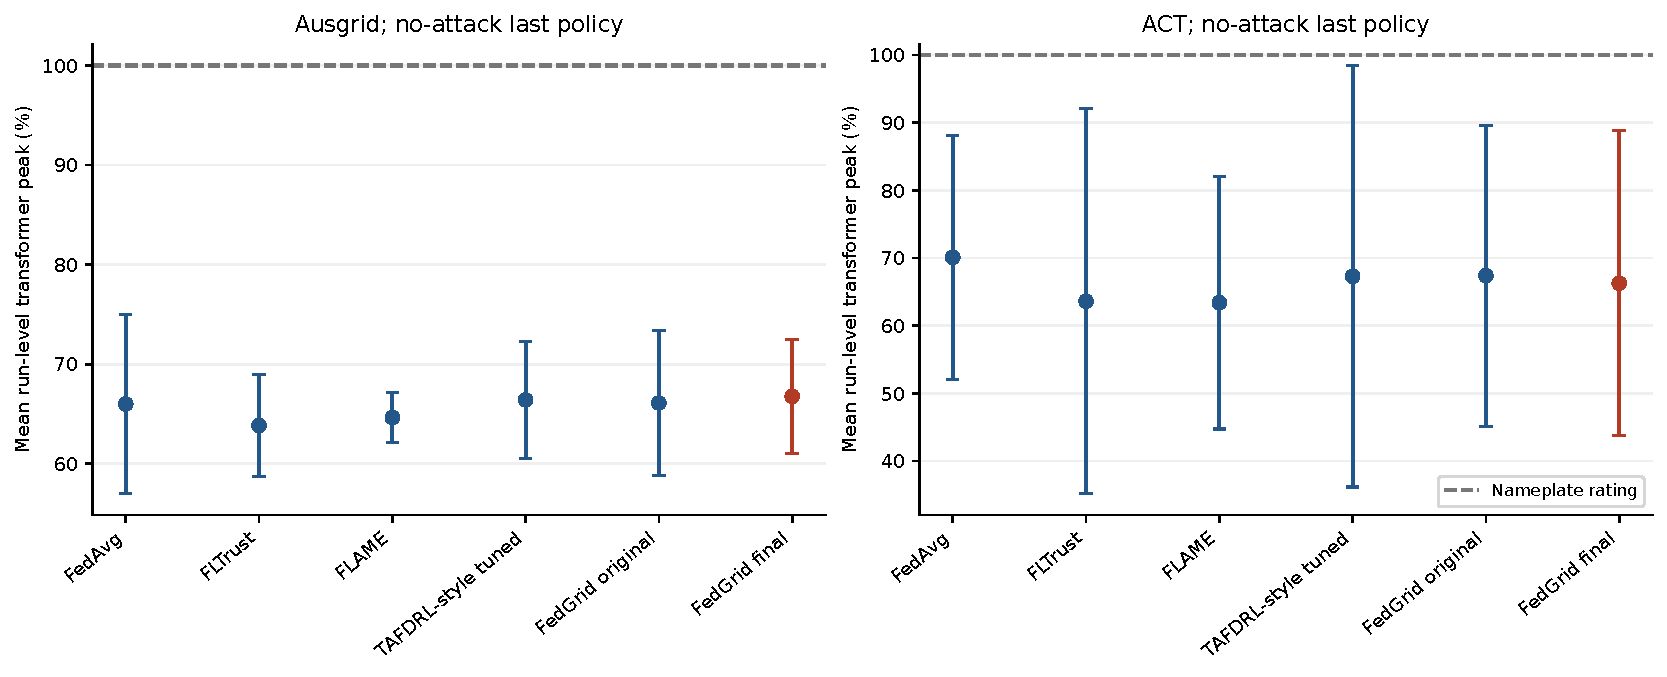
\includegraphics[width=\linewidth]{figures/electrical.pdf}
\caption{Run-level peak transformer loading in no-attack last-policy references, with seed means and 95\% interval half-widths. Ausgrid uses five seeds and ACT three, except the legacy FedAvg transformer statistic has four Ausgrid observations. The dashed line marks nameplate loading; it is not an enforced simulator constraint.}
\label{fig:electrical}
\end{figure}

\subsection{Transfer outcomes with explicit coverage}
Table~\ref{tab:transfer_damage} reports transfer outcomes using five seeds for the final variants and seeds 3--4 for the other configurations. Revision effects use the common-seed differences in Table~\ref{tab:paired_revision}, rather than differences between these unequal aggregate means.

% BEGIN SOURCE: tables/transfer_damage.tex
\begin{table}[htbp]
\centering\small
\caption{Annual bill damage on ACT transfer. Mean $\pm$ 95\% interval half-width [seeds], dollars per household. Transfer coverage differs by method.}
\label{tab:transfer_damage}
\resizebox{\linewidth}{!}{%
\begin{tabular}{lllllll}
\toprule
Method & Flip & Scale & Noise & Normalized & Meter & Reward \\
\midrule
FedAvg & 143.6 $\pm$ 317.5 [2] & 87.5 $\pm$ 1060.1 [2] & 756.3 $\pm$ 920.3 [2] & 842.0 $\pm$ 1124.3 [2] & 9.0 $\pm$ 277.0 [2] & 106.7 $\pm$ 566.9 [2] \\
Median & 110.1 $\pm$ 692.9 [2] & -14.1 $\pm$ 377.8 [2] & -3.5 $\pm$ 255.1 [2] & 190.6 $\pm$ 914.7 [2] & -11.7 $\pm$ 74.6 [2] & 131.9 $\pm$ 217.3 [2] \\
Trimmed mean & 86.4 $\pm$ 47.0 [2] & -20.6 $\pm$ 269.5 [2] & -0.2 $\pm$ 242.8 [2] & 369.2 $\pm$ 136.8 [2] & 16.6 $\pm$ 55.8 [2] & 141.9 $\pm$ 214.2 [2] \\
Krum & -22.8 $\pm$ 1103.8 [2] & -5.5 $\pm$ 827.7 [2] & 49.2 $\pm$ 21.4 [2] & 61.4 $\pm$ 525.0 [2] & -7.6 $\pm$ 816.2 [2] & 20.7 $\pm$ 1027.3 [2] \\
FLTrust & -4.2 $\pm$ 81.5 [2] & 4.3 $\pm$ 70.4 [2] & -35.4 $\pm$ 32.9 [2] & 83.5 $\pm$ 456.3 [2] & 30.0 $\pm$ 15.4 [2] & 61.3 $\pm$ 85.0 [2] \\
FLAME & 66.2 $\pm$ 266.8 [2] & 4.6 $\pm$ 134.9 [2] & 8.0 $\pm$ 371.7 [2] & 26.6 $\pm$ 47.8 [2] & 12.3 $\pm$ 379.3 [2] & -8.3 $\pm$ 52.2 [2] \\
TAFDRL-style & 108.7 $\pm$ 17.6 [2] & 5.8 $\pm$ 207.5 [2] & -4.9 $\pm$ 293.8 [2] & 105.9 $\pm$ 499.9 [2] & 16.3 $\pm$ 35.4 [2] & 7.0 $\pm$ 238.2 [2] \\
TAFDRL-style tuned & 49.9 $\pm$ 29.6 [5] & 28.8 $\pm$ 32.8 [5] & 4.0 $\pm$ 15.7 [5] & 35.8 $\pm$ 98.4 [5] & 17.2 $\pm$ 21.3 [5] & 24.4 $\pm$ 44.9 [5] \\
FedGrid original & 121.6 $\pm$ 310.5 [2] & 0.3 $\pm$ 61.2 [2] & 75.2 $\pm$ 1.8 [2] & 113.5 $\pm$ 42.2 [2] & 29.1 $\pm$ 279.9 [2] & 110.1 $\pm$ 588.4 [2] \\
FedGrid final & 78.9 $\pm$ 47.0 [5] & -12.0 $\pm$ 19.4 [5] & 21.4 $\pm$ 29.1 [5] & -3.3 $\pm$ 60.0 [5] & 28.3 $\pm$ 23.4 [5] & 103.9 $\pm$ 39.6 [5] \\
\bottomrule
\end{tabular}}
\end{table}

% END SOURCE: tables/transfer_damage.tex


\subsection{Compromised share}
Normalized-attack sensitivity uses seed 0 at nominal compromised shares of 10, 20, 30 and 40\%. Trimmed mean and Krum change their assumed faulty count and use share-matched no-attack references; other methods use their seed-0 30\% reference. Final FedGrid has lower observed damage than FedAvg in these cases. Four settings from one seed do not, however, identify a resilience threshold, particularly when a capacity band may contain a compromised majority.

% BEGIN SOURCE: tables/attack_share.tex
\begin{table}[htbp]
\centering\small
\caption{Normalized-attack annual bill damage by nominal compromised share, seed 0 only. Trimmed mean and Krum use share-matched references; other methods use their 30\% no-attack reference.}
\label{tab:attack_share}
\resizebox{\linewidth}{!}{%
\begin{tabular}{lllll}
\toprule
Method & 10\% & 20\% & 30\% & 40\% \\
\midrule
FedAvg & 297.7 [1] & 446.5 [1] & 516.1 [1] & 516.2 [1] \\
Median & 50.4 [1] & 94.0 [1] & 267.9 [1] & 301.3 [1] \\
Trimmed mean & 48.7 [1] & 147.2 [1] & 192.5 [1] & 394.9 [1] \\
Krum & 75.6 [1] & 76.9 [1] & -37.5 [1] & 110.9 [1] \\
FLTrust & -42.8 [1] & -41.4 [1] & -32.9 [1] & -7.9 [1] \\
FLAME & -21.3 [1] & 31.7 [1] & -25.5 [1] & 39.1 [1] \\
TAFDRL-style & 25.1 [1] & 37.8 [1] & 12.6 [1] & 121.8 [1] \\
TAFDRL-style tuned & -6.4 [1] & -9.9 [1] & -35.0 [1] & 13.5 [1] \\
FedGrid original & 23.9 [1] & 79.8 [1] & 94.8 [1] & 105.9 [1] \\
FedGrid final & 16.6 [1] & 18.7 [1] & -19.4 [1] & 17.9 [1] \\
\bottomrule
\end{tabular}}
\end{table}

% END SOURCE: tables/attack_share.tex

\begin{figure}[htbp]
\centering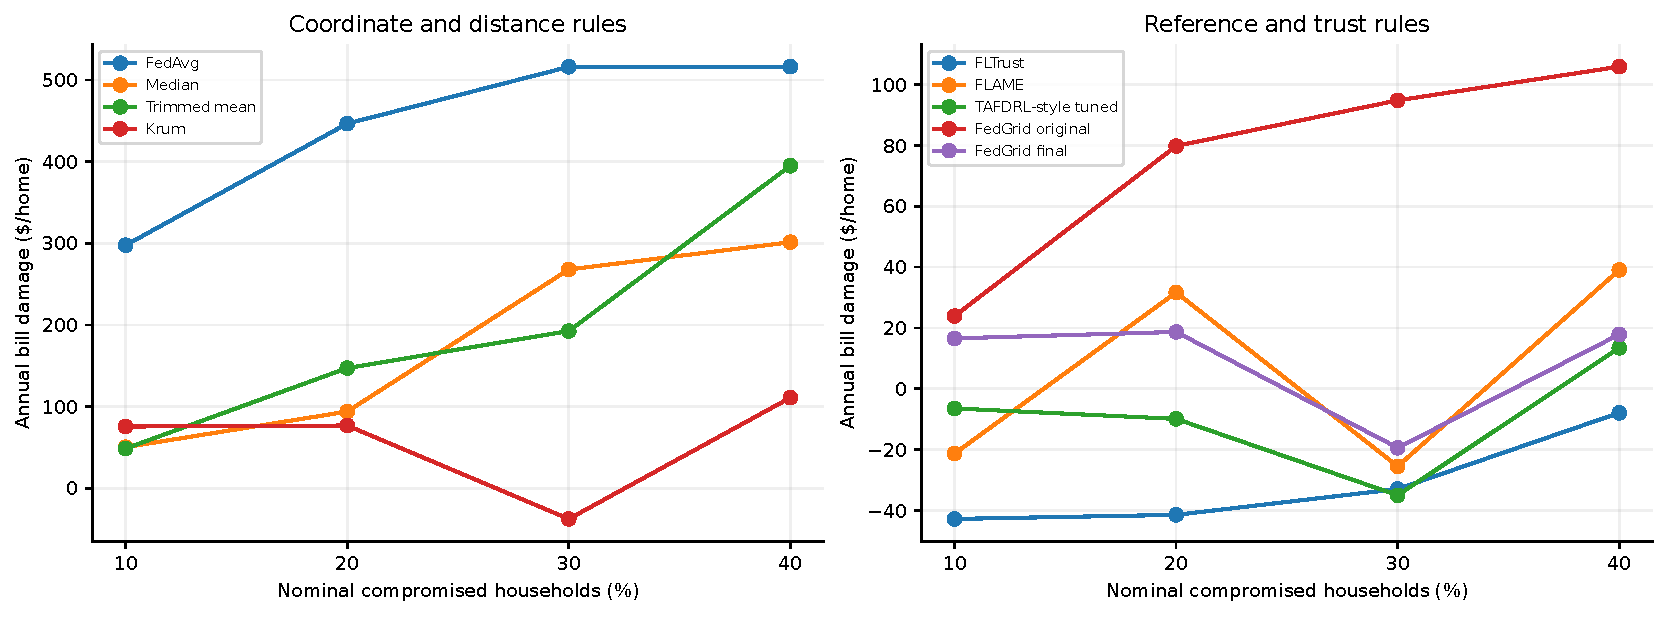
\includegraphics[width=\linewidth]{figures/attack_share.pdf}
\caption{Normalized-attack damage versus nominal compromised share, seed 0 only. Separate panels improve readability; vertical scales differ. Each point is a single experimental difference with no seed uncertainty interval.}
\label{fig:shares}
\end{figure}

\subsection{Ablation and operation order}
Each original-method ablation removes clipping, grouping or trust separately. Without clipping, Normalized damage is lower in these three seeds; removing grouping or trust does not reproduce the final configuration's outcome. The final configuration jointly changes filter order and clipping bound. These comparisons indicate an interaction worth examining, but do not isolate the cause of the combined revision's improvement.

% BEGIN SOURCE: tables/ablation.tex
\begin{table}[htbp]
\centering\small
\caption{Normalized-attack damage and logged honest rejection for the original FedGrid ablations and final variant, seeds 0--2. The final variant changes both filter order and clipping multiplier; it is not a one-factor ablation.}
\label{tab:ablation}
\resizebox{\linewidth}{!}{%
\begin{tabular}{lll}
\toprule
Variant & Damage (\$/home/yr) & Honest rejection (\%) \\
\midrule
original & 89.9 $\pm$ 25.7 [3] & 4.9 $\pm$ 2.9 [3] \\
without\_clip & -0.3 $\pm$ 102.8 [3] & 6.8 $\pm$ 3.0 [3] \\
without\_groups & 125.0 $\pm$ 90.5 [3] & 3.2 $\pm$ 3.1 [3] \\
without\_trust & 111.0 $\pm$ 248.1 [3] & 9.2 $\pm$ 8.4 [3] \\
final & -9.3 $\pm$ 130.2 [3] & 6.3 $\pm$ 5.2 [3] \\
\bottomrule
\end{tabular}}
\end{table}

% END SOURCE: tables/ablation.tex

\begin{figure}[htbp]
\centering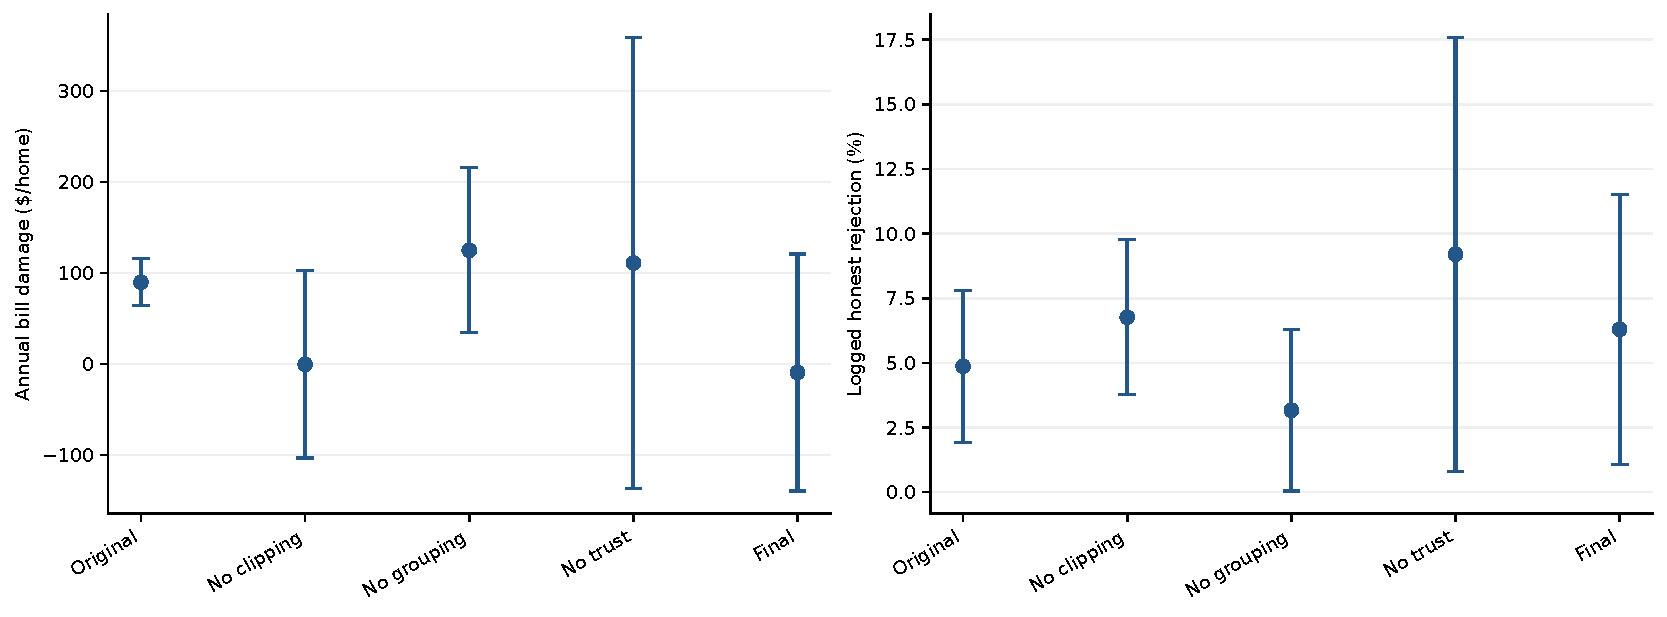
\includegraphics[width=\linewidth]{figures/ablation.pdf}
\caption{Original FedGrid ablations and final variant under Normalized attack, seeds 0--2. Error bars are unadjusted 95\% Student-$t$ intervals. Rejection refers to the logged admission mask. The final variant is a combined revision, not a single-factor ablation.}
\label{fig:ablation}
\end{figure}

\subsection{Communication faults, feeder size and voltage stress}
Table~\ref{tab:sensitivity} pairs each scenario with its same-method no-attack reference. Final FedGrid's Normalized damage is approximately $-\$18$ under the specified message faults, \$37 on feeder O and $-\$12$ at 1.02\,pu. Each is a single-seed sensitivity observation. Negative differences do not establish a benefit from faults or attacks. The large trimmed-mean damage under message faults is also consistent with a possible interaction between received-population size and share-dependent trimming, which the present cases do not isolate.

% BEGIN SOURCE: tables/sensitivity.tex
\begin{table}[htbp]
\centering\small
\caption{Normalized-attack damage under message faults, feeder O and 1.02 pu supply, seed 0. A dash means unavailable, not zero. Damage is in dollars per household per year, using the same variant and method no-attack reference.}
\label{tab:sensitivity}
\resizebox{\linewidth}{!}{%
\begin{tabular}{llll}
\toprule
Method & Lost/delayed (\$/home/yr) & Feeder O (\$/home/yr) & 1.02 pu (\$/home/yr) \\
\midrule
FedAvg & 529.2 [1] & 515.5 [1] & 614.6 [1] \\
Median & 261.9 [1] & -- & -- \\
Trimmed mean & 1224.0 [1] & -- & -- \\
Krum & -29.4 [1] & -- & -- \\
FLTrust & -37.0 [1] & 12.3 [1] & 32.4 [1] \\
FLAME & 2.3 [1] & 88.4 [1] & 25.0 [1] \\
TAFDRL-style & 10.5 [1] & -- & -- \\
TAFDRL-style tuned & 38.7 [1] & -- & -- \\
FedGrid original & 59.9 [1] & 137.9 [1] & -- \\
FedGrid final & -18.3 [1] & 36.7 [1] & -11.6 [1] \\
\bottomrule
\end{tabular}}
\end{table}

% END SOURCE: tables/sensitivity.tex

\begin{figure}[htbp]
\centering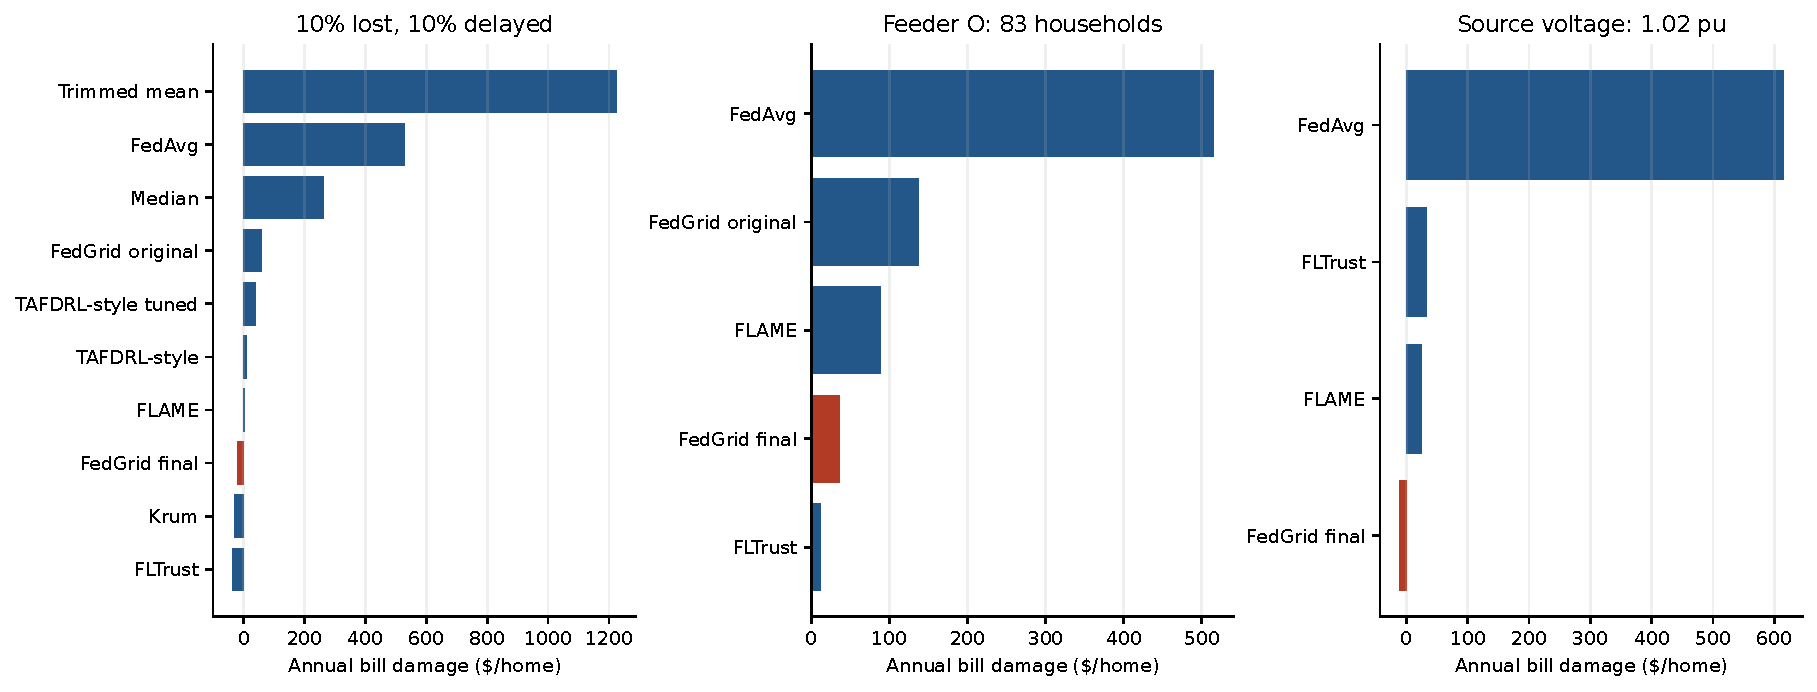
\includegraphics[width=\linewidth]{figures/sensitivity.pdf}
\caption{Normalized-attack damage in three sensitivity cases, seed 0. All-home annual bill differences use matched scenario references. Panels have different horizontal scales. Missing method--scenario combinations are not imputed.}
\label{fig:sensitivity}
\end{figure}

\subsection{Validation trajectories}
The trajectories show the mean and observed minimum--maximum range over seeds 0--2. They track validation-week cost plus the curtailment penalty, not annual evaluation bills. Reward-poisoned policies are assessed with ordinary observations after learning from reversed rewards. These are development diagnostics from the existing runs, not independent validation.
\begin{figure}[htbp]
\centering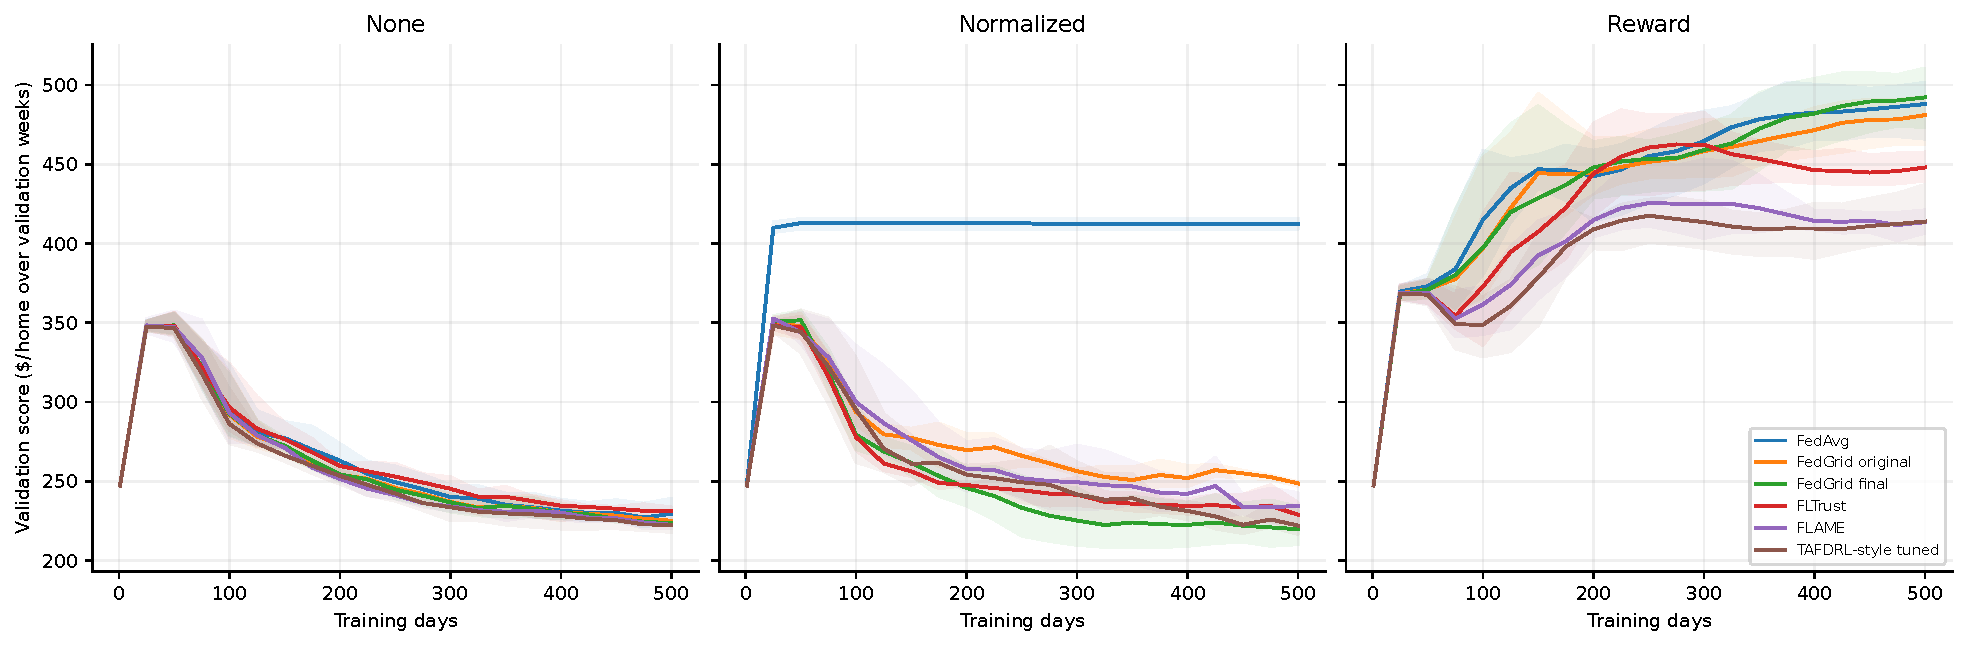
\includegraphics[width=\linewidth]{figures/training_curves.pdf}
\caption{Validation trajectories under no attack, Normalized attack and reward poisoning. Lines are three-seed means and shading is the observed seed range, not a confidence interval. Each panel shows validation objective values over training days.}
\label{fig:training}
\end{figure}

\subsection{Computational measurements}
The benchmark instantiates one household's actor and critics, containing 54,916 network values including local output layers. Table~\ref{tab:device} gives three repeated single-core trials on one Intel i7-10610U laptop; Linux peak-memory values are expressed in MiB. Shared-layer payload figures exclude local layers, optimiser state, target networks, protocol overhead and the reference learner. Server aggregation, transfers and the target embedded device would require separate deployment measurements.

% BEGIN SOURCE: tables/device.tex
\begin{table}[htbp]
\centering\small
\caption{Archived single-core laptop measurements (Intel i7-10610U). Three repeated timing trials on one device; these are not three independent hardware platforms.}
\label{tab:device}
\resizebox{\linewidth}{!}{%
\begin{tabular}{llll}
\toprule
Trial & Decision (ms) & Gradient step (ms) & Peak process memory (MiB) \\
\midrule
1 & 0.06 & 4.4 & 353 \\
2 & 0.04 & 4.1 & 356 \\
3 & 0.05 & 4.2 & 356 \\
\bottomrule
\end{tabular}}
\end{table}

% END SOURCE: tables/device.tex


\subsection{Computational reproducibility}
The accompanying artifacts contain per-seed outcomes, plotted values, analysis scripts and SHA-256 manifests. Statistical exports retain seed pairing and raw and adjusted p-values. Imputation records retain recipient and donor timestamps, their partitions and the denominators used for overlap fractions. Together, these records support reproduction of the analysis of existing experiments. Public archival identifiers and access terms have not been assigned.

\subsection{Audit of imputation donor overlap}
The donor audit reads raw ACT profiles and reconstructs the first observed value selected for each missing half hour by the fixed nearest-day rule. Reconstructed values are checked against the processed load and solar files at their stored precision. The audit uses the seed-zero evaluation street and its disjoint reference households. A profile cell denotes one household's load or solar value at one half hour; its denominator is distinct from a trajectory count or a household bill.

In the 36-home evaluation street, 2,004 training cells use donors from another partition, representing 0.259\% of training load-and-solar cells. Of these, 1,540 use evaluation-week donors. The reference street also contains 1,540 training cells with evaluation-week donors. The copied fraction alone does not bound its effect on policy selection or annual bills. A controlled rerun with partition-isolated preprocessing is needed to estimate that effect; this audit quantifies the overlap without correcting the reported experiments.

% BEGIN SOURCE: tables/imputation_audit.tex
\begin{table}[htbp]
\centering\small
\caption{Read-only ACT imputation donor audit for the 36-home evaluation and reference streets. Counts pool load and solar half-hour cells. Cross-partition percentages use all profile cells in the recipient partition, not only filled cells. Copied evaluation data are a qualification of the existing evidence; no policy rerun is implied.}
\label{tab:imputation_audit}
\resizebox{\linewidth}{!}{%
\begin{tabular}{llrrrr}
\toprule
Street & Recipient partition & Filled cells & Cross-partition cells & Cross-partition (\%) & Donors from test \\
\midrule
Evaluation & train & 12,180 & 2,004 & 0.259 & 1,540 \\
Evaluation & validation & 2,980 & 388 & 0.229 & 0 \\
Evaluation & test & 3,168 & 396 & 0.126 & 2,772 \\
Reference & train & 12,748 & 2,000 & 0.258 & 1,540 \\
Reference & validation & 1,936 & 292 & 0.172 & 0 \\
Reference & test & 3,748 & 480 & 0.153 & 3,268 \\
\bottomrule
\end{tabular}}
\end{table}

% END SOURCE: tables/imputation_audit.tex


\subsection{Exact paired statistical audit}
Two-sided exact Wilcoxon signed-rank tests compare five-seed Ausgrid damage. The robust-comparator family contains final FedGrid against FLTrust, FLAME and tuned TAFDRL-style across six attacks (18 tests). The revision family contains final against original FedGrid across the same six attacks. Holm adjustment is applied separately within each family. These are exploratory tests on already observed data, not a prospectively registered analysis.

All comparisons have nonzero differences and no tied absolute ranks. For five such pairs, the smallest attainable two-sided exact p-value is $2/2^5=0.0625$; a value below 0.05 is therefore unattainable even before adjustment. The Normalized final-minus-original comparison has exact p-value 0.0625 and six-test adjusted p-value 0.375. A descriptive Student-$t$ interval may exclude zero because the interval and rank test use different assumptions and formulations. Both results are reported with their scope, and all pair differences and p-values are exported as CSV.

% BEGIN SOURCE: tables/exact_statistics.tex
\begin{table}[htbp]
\centering\small
\caption{Exploratory two-sided exact paired Wilcoxon tests on five Ausgrid seeds. Differences are final FedGrid minus the comparator. Holm adjustment uses 18 tests for robust comparators and six for the original-method revision; no adjusted test rejects at 0.05.}
\label{tab:exact_statistics}
\begin{tabular}{llrrr}
\toprule
Comparator & Attack & Mean difference (\$/yr) & Exact $p$ & Holm $p$ \\
\midrule
FLTrust & Flip & 68.1 & 0.0625 & 1.000 \\
FLTrust & Scale & -12.9 & 0.0625 & 1.000 \\
FLTrust & Noise & 33.0 & 0.1250 & 1.000 \\
FLTrust & Normalized & -11.8 & 0.8125 & 1.000 \\
FLTrust & Meter & 5.9 & 1.0000 & 1.000 \\
FLTrust & Reward & 42.8 & 0.0625 & 1.000 \\
FLAME & Flip & 14.0 & 0.1875 & 1.000 \\
FLAME & Scale & -19.5 & 0.3125 & 1.000 \\
FLAME & Noise & 17.3 & 0.3125 & 1.000 \\
FLAME & Normalized & -31.8 & 0.3125 & 1.000 \\
FLAME & Meter & 15.3 & 0.4375 & 1.000 \\
FLAME & Reward & 64.7 & 0.0625 & 1.000 \\
TAFDRL-style tuned & Flip & 29.7 & 0.3125 & 1.000 \\
TAFDRL-style tuned & Scale & -29.6 & 0.1250 & 1.000 \\
TAFDRL-style tuned & Noise & 22.6 & 0.0625 & 1.000 \\
TAFDRL-style tuned & Normalized & -27.7 & 0.6250 & 1.000 \\
TAFDRL-style tuned & Meter & 18.9 & 0.6250 & 1.000 \\
TAFDRL-style tuned & Reward & 42.4 & 0.1250 & 1.000 \\
FedGrid original & Flip & -10.4 & 0.3125 & 1.000 \\
FedGrid original & Scale & -5.3 & 0.6250 & 1.000 \\
FedGrid original & Noise & -28.4 & 0.0625 & 0.375 \\
FedGrid original & Normalized & -76.8 & 0.0625 & 0.375 \\
FedGrid original & Meter & 13.6 & 0.4375 & 1.000 \\
FedGrid original & Reward & 14.6 & 0.4375 & 1.000 \\
\bottomrule
\end{tabular}
\end{table}

% END SOURCE: tables/exact_statistics.tex


\subsection{Training duration and FedProx coefficient}
Table~\ref{tab:extended_clean} reports all 30 current clean-learning runs: the 500-day and 1000-day settings for four learned baselines, plus the two additional FedProx coefficients. Each cell uses three seeds and the same validation-selected retention rule. These comparisons describe the available archive; they do not extend the attack evaluation to 1000 days or establish convergence.

% BEGIN SOURCE: tables/extended_clean.tex
\begin{table}[htbp]
\centering\small
\caption{All 30 clean-learning runs: duration and FedProx-coefficient comparisons with validation-selected actors. Entries are mean $\pm$ 95\% interval half-width [seeds]. Bills and curtailment are per household annually; cycles are fleet-equivalent, and MSL charging is a street total.}
\label{tab:extended_clean}
\resizebox{\linewidth}{!}{%
\begin{tabular}{lllllll}
\toprule
Method & Days & $\mu$ & Bill (\$/yr) & Curtailment (kWh/yr) & Cycles/yr & MSL charge (kWh) \\
\midrule
Local SAC & 500 & -- & 963.8 $\pm$ 61.2 [3] & 134.8 $\pm$ 49.4 [3] & 247.4 $\pm$ 39.4 [3] & 13307.6 $\pm$ 2085.6 [3] \\
Local SAC & 1000 & -- & 926.9 $\pm$ 66.4 [3] & 122.6 $\pm$ 32.2 [3] & 248.6 $\pm$ 33.3 [3] & 13735.5 $\pm$ 1215.0 [3] \\
FedAvg & 500 & -- & 954.3 $\pm$ 79.0 [3] & 144.6 $\pm$ 89.9 [3] & 255.9 $\pm$ 48.6 [3] & 12735.2 $\pm$ 4074.3 [3] \\
FedAvg & 1000 & -- & 902.0 $\pm$ 74.0 [3] & 122.5 $\pm$ 17.0 [3] & 262.8 $\pm$ 3.3 [3] & 13503.5 $\pm$ 672.5 [3] \\
FedProx & 500 & 0.01 & 947.3 $\pm$ 65.2 [3] & 153.5 $\pm$ 84.8 [3] & 252.7 $\pm$ 38.8 [3] & 12396.6 $\pm$ 3452.8 [3] \\
FedProx & 1000 & 0.01 & 890.4 $\pm$ 119.1 [3] & 138.5 $\pm$ 28.8 [3] & 255.2 $\pm$ 11.0 [3] & 12617.5 $\pm$ 693.8 [3] \\
Central SAC & 500 & -- & 879.1 $\pm$ 117.7 [3] & 137.9 $\pm$ 160.3 [3] & 277.7 $\pm$ 34.9 [3] & 13872.7 $\pm$ 4775.5 [3] \\
Central SAC & 1000 & -- & 810.1 $\pm$ 142.8 [3] & 162.8 $\pm$ 166.1 [3] & 265.4 $\pm$ 85.3 [3] & 12674.2 $\pm$ 6357.2 [3] \\
FedProx & 500 & 0.001 & 944.4 $\pm$ 61.8 [3] & 131.9 $\pm$ 58.5 [3] & 258.2 $\pm$ 25.1 [3] & 13271.1 $\pm$ 601.7 [3] \\
FedProx & 500 & 0.1 & 950.6 $\pm$ 10.9 [3] & 141.0 $\pm$ 20.1 [3] & 255.6 $\pm$ 48.4 [3] & 12815.9 $\pm$ 1875.7 [3] \\
\bottomrule
\end{tabular}}
\end{table}

% END SOURCE: tables/extended_clean.tex


\subsection{Deterministic baseline context}
Table~\ref{tab:all_baselines} retains the idle, rule and perfect-foresight MPC outcomes for Ausgrid, ACT and the 1.02\,pu stress scenario. In particular, low MPC bills coexist with observed transformer loading above nameplate in ACT and voltage stress. Missing legacy transformer measurements remain missing.

% BEGIN SOURCE: tables/all_baselines.tex
\begin{table}[htbp]
\centering\small
\caption{All archived deterministic baselines, in Australian dollars per household per year and curtailed kWh per household per year. Electrical metrics describe observed evaluation intervals. Missing legacy transformer measurements are shown as dashes.}
\label{tab:all_baselines}
\resizebox{\linewidth}{!}{%
\begin{tabular}{lllllll}
\toprule
Scenario & Controller & Bill (\$/yr) & Curtailment (kWh/yr) & Over 253 V (\%) & Max V & Peak loading (\%) \\
\midrule
Ausgrid 1.00 pu & Idle & 1457.78 & 537.74 & 0.000 & 252.92 & -- \\
Ausgrid 1.00 pu & Rule & 952.96 & 473.18 & 0.000 & 252.92 & -- \\
Ausgrid 1.00 pu & Perfect-foresight MPC & 590.95 & 62.87 & 0.000 & 252.93 & -- \\
ACT 1.00 pu & Idle & 1864.79 & 329.74 & 0.000 & 251.85 & 87.95 \\
ACT 1.00 pu & Rule & 1198.77 & 231.71 & 0.000 & 251.85 & 84.77 \\
ACT 1.00 pu & Perfect-foresight MPC & 875.94 & 19.04 & 0.000 & 252.65 & 109.57 \\
Ausgrid 1.02 pu & Idle & 1500.18 & 1027.39 & 6.880 & 254.49 & 73.76 \\
Ausgrid 1.02 pu & Rule & 988.73 & 886.22 & 4.450 & 255.52 & 73.40 \\
Ausgrid 1.02 pu & Perfect-foresight MPC & 590.65 & 64.72 & 3.030 & 254.38 & 111.50 \\
\bottomrule
\end{tabular}}
\end{table}

% END SOURCE: tables/all_baselines.tex


\subsection{Electrical outcomes under all principal attacks}
Table~\ref{tab:attack_electrical} takes the maximum available run-level voltage and transformer metrics over each method's six principal attacks. This extends the no-attack reference display without selecting only favourable scenarios. Different cells may reach their maxima in different runs, and missing legacy measurements are excluded rather than imputed. The accompanying CSV records method, setting, seed, attack and source for each run.

% BEGIN SOURCE: tables/attack_electrical.tex
\begin{table}[htbp]
\centering\small
\caption{Maximum observed run-level electrical metrics over all six attacks at 30\% nominal compromise: five Ausgrid seeds and three ACT seeds. Each cell is a maximum across available logs; different maxima may arise from different attacks or seeds. Ausgrid transformer measurements cover 26/30 runs for FedAvg, median, trimmed mean and Krum, and 30/30 otherwise; ACT covers 18/18 throughout. All voltage metrics have full coverage. Missing measurements are excluded, never set to zero; per-run inputs are retained in the CSV.}
\label{tab:attack_electrical}
\resizebox{\linewidth}{!}{%
\begin{tabular}{lllllll}
\toprule
Method & Ausgrid over 253 V (\%) & Ausgrid max V & Ausgrid peak (\%) & ACT over 253 V (\%) & ACT max V & ACT peak (\%) \\
\midrule
FedAvg & 0.120 & 253.14 & 113.84 & 0.000 & 251.96 & 94.49 \\
Median & 0.000 & 252.83 & 84.25 & 0.070 & 253.46 & 76.71 \\
Trimmed mean & 0.000 & 252.82 & 75.67 & 0.000 & 252.62 & 78.57 \\
Krum & 0.000 & 252.71 & 70.86 & 0.000 & 252.70 & 84.48 \\
FLTrust & 0.000 & 252.81 & 73.49 & 0.000 & 251.97 & 74.36 \\
FLAME & 0.010 & 253.27 & 73.19 & 0.000 & 252.03 & 73.54 \\
TAFDRL-style & 0.090 & 253.46 & 76.45 & 0.000 & 252.27 & 79.20 \\
TAFDRL-style tuned & 0.070 & 253.50 & 77.87 & 0.000 & 252.34 & 77.94 \\
FedGrid original & 0.000 & 252.91 & 74.86 & 0.000 & 252.92 & 83.60 \\
FedGrid final & 0.010 & 253.19 & 72.29 & 0.000 & 252.30 & 76.24 \\
\bottomrule
\end{tabular}}
\end{table}

% END SOURCE: tables/attack_electrical.tex


\subsection{Household heterogeneity in recorded rejection}
Table~\ref{tab:heterogeneity} compares honest homes at the lowest or highest solar-capacity sextile thresholds with the remaining honest homes, under no attack and Normalized. Thresholds use the rounded capacities printed in each street's logs, with ties retained. Per-home rejection rates are also rounded, so the resulting means are retrospective filter diagnostics rather than precise measurements of influence. The maximum-household column averages the most-rejected household within each run; it is not a worst case over all runs.

% BEGIN SOURCE: tables/heterogeneity.tex
\begin{table}[htbp]
\centering\small
\caption{Logged honest rejection (\%) by solar-capacity stratum, no attack and Normalized, seeds 0--4 where available. Unusual homes fall at or beyond the lowest/highest sextile thresholds of rounded street capacities; ties may enlarge the stratum. Per-home rates are rounded in the logs. Entries are mean $\pm$ 95\% interval half-width [observed seeds]. The last column averages the maximum household rejection within each run; these are filter diagnostics, not effective-influence measurements.}
\label{tab:heterogeneity}
\resizebox{\linewidth}{!}{%
\begin{tabular}{llllll}
\toprule
Method & Condition & Overall (\%) & Unusual PV (\%) & Other PV (\%) & Mean run maximum (\%) \\
\midrule
Krum & None & 97.2 $\pm$ 0.0 [4] & 99.7 $\pm$ 0.5 [4] & 95.3 $\pm$ 0.4 [4] & 100.0 $\pm$ 0.0 [4] \\
Krum & Normalized & 96.4 $\pm$ 0.1 [4] & 100.0 $\pm$ 0.0 [4] & 93.3 $\pm$ 0.9 [4] & 100.0 $\pm$ 0.0 [4] \\
FLTrust & None & 31.6 $\pm$ 4.8 [5] & 41.9 $\pm$ 6.7 [5] & 23.4 $\pm$ 3.6 [5] & 70.8 $\pm$ 9.1 [5] \\
FLTrust & Normalized & 16.2 $\pm$ 4.0 [5] & 20.4 $\pm$ 6.2 [5] & 12.5 $\pm$ 2.2 [5] & 37.3 $\pm$ 12.6 [5] \\
FLAME & None & 47.0 $\pm$ 0.2 [5] & 57.1 $\pm$ 2.3 [5] & 38.8 $\pm$ 1.6 [5] & 99.7 $\pm$ 0.4 [5] \\
FLAME & Normalized & 46.3 $\pm$ 2.1 [5] & 56.5 $\pm$ 8.0 [5] & 37.4 $\pm$ 5.7 [5] & 98.9 $\pm$ 0.5 [5] \\
TAFDRL-style & None & 8.5 $\pm$ 0.8 [5] & 10.8 $\pm$ 2.1 [5] & 6.6 $\pm$ 2.0 [5] & 48.0 $\pm$ 6.9 [5] \\
TAFDRL-style & Normalized & 31.1 $\pm$ 3.7 [5] & 42.4 $\pm$ 6.6 [5] & 21.4 $\pm$ 6.0 [5] & 88.6 $\pm$ 4.8 [5] \\
TAFDRL-style tuned & None & 20.4 $\pm$ 2.2 [5] & 32.5 $\pm$ 2.1 [5] & 10.6 $\pm$ 4.3 [5] & 99.1 $\pm$ 0.7 [5] \\
TAFDRL-style tuned & Normalized & 53.0 $\pm$ 7.7 [5] & 67.6 $\pm$ 9.6 [5] & 40.1 $\pm$ 13.1 [5] & 100.0 $\pm$ 0.0 [5] \\
FedGrid original & None & 3.2 $\pm$ 0.7 [5] & 2.7 $\pm$ 1.3 [5] & 3.5 $\pm$ 1.4 [5] & 34.5 $\pm$ 12.2 [5] \\
FedGrid original & Normalized & 4.6 $\pm$ 1.8 [5] & 5.0 $\pm$ 5.2 [5] & 4.4 $\pm$ 3.4 [5] & 29.0 $\pm$ 9.9 [5] \\
FedGrid final & None & 6.2 $\pm$ 1.3 [5] & 6.0 $\pm$ 0.8 [5] & 6.2 $\pm$ 2.7 [5] & 48.2 $\pm$ 14.9 [5] \\
FedGrid final & Normalized & 6.5 $\pm$ 3.8 [5] & 9.8 $\pm$ 10.2 [5] & 4.1 $\pm$ 3.2 [5] & 41.7 $\pm$ 30.6 [5] \\
\bottomrule
\end{tabular}}
\end{table}

% END SOURCE: tables/heterogeneity.tex


\subsection{Full selection-setting evidence}
Table~\ref{tab:selection_settings} includes the later clipping settings, earlier household-trust settings and four TAFDRL-style configurations. The rejection pools and tuning attack sets differ as described in Section~\ref{sec:selection}. FedGrid's 40\% Normalized validation damage is reported for completeness and did not enter the four-attack ranking. The archived historical flags and choice reports remain unchanged.

% BEGIN SOURCE: tables/selection_settings.tex
\begin{table}[htbp]
\centering\small
\caption{Completed later settings and TAFDRL-style tuning on validation data. Worst damage uses the available update attacks (four for FedGrid; two for tuned TAFDRL-style). Recorded honest rejection pools all available 30\% runs, including no attack; the two families therefore have different pools. TAFDRL-style tuning fixes minimum trust at 0.35. The 40\% column is three-seed Normalized validation damage for FedGrid, excluded from the ranking criterion. Values follow the historical one-decimal reporting and are not annual evaluation damage.}
\label{tab:selection_settings}
\resizebox{\linewidth}{!}{%
\begin{tabular}{lllllll}
\toprule
Family & Setting & Worst validation damage (\$) & Honest rejection (\%) & Rejection runs & Attacks & 40\% damage (\$) \\
\midrule
Final FedGrid & 3 bands, z 2.5 & 14.5 & 3.4 & 15 & 4 & -5.9 \\
Final FedGrid & 2 bands & 20.9 & 1.7 & 15 & 4 & -9.1 \\
Final FedGrid & 4 bands & 23.3 & 2.2 & 15 & 4 & -5.3 \\
Final FedGrid & z 2.0 & 17.9 & 5.9 & 15 & 4 & 1.2 \\
Final FedGrid & z 3.0 & 15.8 & 2.6 & 15 & 4 & -9.7 \\
Earlier home trust & 3 bands, z 2.5 & 6.2 & 30.8 & 15 & 4 & 4.9 \\
Earlier home trust & 2 bands & 4.9 & 28.9 & 15 & 4 & 8.1 \\
Earlier home trust & 4 bands & 5.4 & 29.2 & 15 & 4 & 10.5 \\
Earlier home trust & z 2.0 & 0.5 & 32.4 & 15 & 4 & 7.8 \\
Earlier home trust & z 3.0 & 1.1 & 29.9 & 15 & 4 & -4.3 \\
TAFDRL-style & lambda 1, level .99 & 19.2 & 19.4 & 9 & 2 & -- \\
TAFDRL-style & lambda 1, level .999 & 22.0 & 10.4 & 9 & 2 & -- \\
TAFDRL-style & lambda 2, level .99 & 10.5 & 28.6 & 9 & 2 & -- \\
TAFDRL-style & lambda 2, level .999 & 17.8 & 14.7 & 9 & 2 & -- \\
\bottomrule
\end{tabular}}
\end{table}

% END SOURCE: tables/selection_settings.tex


% END SOURCE: sections/appendix.tex

\end{document}
